% The TCRen2 descriptor catalogue: hierarchy, classification, formulas, derivations.
% Hand-written prose; every count and every table row comes from appendix/generated/,
% emitted by scripts/gen_appendix.py from the catalogue itself.  2026-09-02
\documentclass[11pt,a4paper]{article}

\usepackage[T1]{fontenc}
\usepackage[utf8]{inputenc}
\usepackage{newtxtext,newtxmath}   % no amssymb: newtxmath provides those symbols and the two clash
\usepackage[margin=2.4cm]{geometry}
\usepackage{amsmath}
\usepackage{array}
\usepackage{booktabs}
\usepackage{longtable}
\usepackage{graphicx}
\usepackage{microtype}
\usepackage{tikz}
\usetikzlibrary{arrows.meta,positioning,decorations.pathmorphing,patterns,calc}
\usepackage[colorlinks,linkcolor=black,citecolor=black,urlcolor=blue!55!black]{hyperref}
\usepackage[capitalise,noabbrev]{cleveref}

% GENERATED by scripts/gen_appendix.py -- do not edit.
\newcommand{\tcrenVersion}{3.0.0}
\newcommand{\nDesc}{164}
\newcommand{\nFamilies}{6}
\newcommand{\nNoReceptor}{5}
\newcommand{\nFlagged}{33}
\newcommand{\nFamPlacement}{31}
\newcommand{\nFamInterface}{26}
\newcommand{\nFamTopology}{70}
\newcommand{\nFamEnergetics}{15}
\newcommand{\nFamPotts}{5}
\newcommand{\nFamKinetics}{17}
\newcommand{\nInvGeometric}{65}
\newcommand{\nInvCompositional}{64}
\newcommand{\nInvCategorical}{1}
\newcommand{\nInvTopological}{14}
\newcommand{\nInvEnergetic}{20}
\newcommand{\nOpFrame}{31}
\newcommand{\nOpCount}{49}
\newcommand{\nOpMoment}{19}
\newcommand{\nOpHill}{19}
\newcommand{\nOpHomology}{10}
\newcommand{\nOpSpectral}{9}
\newcommand{\nOpCorrelation}{6}
\newcommand{\nOpPotential}{19}
\newcommand{\nOpWork}{2}


\newcommand{\dsc}[1]{\texttt{#1}}
\newcommand{\obj}[1]{\ensuremath{\mathcal{#1}}}
\setlength{\parskip}{2pt}

\title{\bfseries The TCRen2 descriptor catalogue\\[2pt]
\large hierarchy, classification, formulas and derivations}
\author{\normalsize \texttt{tcren} \tcrenVersion\ --- \nDesc\ descriptors in \nFamilies\ families}
\date{\normalsize 2 September 2026}

\begin{document}
\maketitle

\begin{abstract}
\noindent
This appendix documents every descriptor \texttt{tcren} computes from a TCR--pMHC structure. It is
organised around a claim: the \nDesc\ descriptors are not \nDesc\ ideas. They are a small set of
\emph{operators} applied to a smaller set of \emph{objects}, each object a strict reduction of the
atomic coordinates. Nine operators and eight objects account for the whole catalogue, and naming
them makes three things visible that the family listing hides --- which descriptors can be
redundant with which (only within a reduction step), which are exactly determined by others, and
which are invariant under what. Nineteen descriptors spread over four families turn out to be one
formula, the Hill number, applied to seven different probability vectors at three orders. Section
\ref{sec:classes} treats MHC class I and class II, which condition several formulas and are
unevenly represented in the corpus. Nothing here is fitted: every descriptor is a deterministic
function of one structure.
\end{abstract}

\tableofcontents

% =================================================================================================
\section{Scope}

A descriptor is a function $f : \mathcal{S} \to \mathbb{R}$ from one annotated TCR--pMHC structure
to one number. Annotation means chain typing, CDR region markup and, for the MHC-facing columns,
groove region markup; nothing else is required, and in particular no alignment to a reference and
no prior canonicalisation of the input orientation. Each $f$ carries a unit, an invariance class
and, where something is known about its behaviour, a \texttt{STATUS} flag. \Cref{sec:catalogue}
lists all \nDesc\ with their definitions; \cref{sec:status} lists the \nFlagged\ flagged ones.

Three properties hold catalogue-wide and are assumed everywhere below.

\begin{description}
\item[No fitted parameter.] No descriptor reads a label, a training set or a coefficient estimated
  from one. The statistical potentials are derived once from a structural database and shipped; the
  Potts couplings likewise. A descriptor's value on a structure does not depend on what else was in
  the batch.
\item[Rigid-motion invariance.] Every descriptor is invariant under the action of $SE(3)$ on the
  input coordinates. The frame-referred quantities of \cref{sec:frame} achieve this by refitting
  their frame from the structure rather than inheriting one, so two copies of a complex in different
  laboratory orientations give identical rows.
\item[Undefined is \texttt{NaN}, never zero.] A descriptor with no support returns \texttt{NaN}. A
  contact order over one contacted residue, a standoff height over a face with no void, a stiffness
  over two springs: each is undefined, and $0$ would rank as an extreme rather than as a missing
  value.
\end{description}

% =================================================================================================
\section{The hierarchy: a chain of reductions}
\label{sec:hierarchy}

The six \emph{families} --- placement, interface, topology, energetics, potts, kinetics --- record
which pass of which command produces a descriptor. That is a fact about the software. The fact
about the science is which \emph{object} the descriptor reads, and the objects form a chain in
which each step discards information irreversibly (\cref{fig:reduction}).

\begin{figure}[t]
\centering
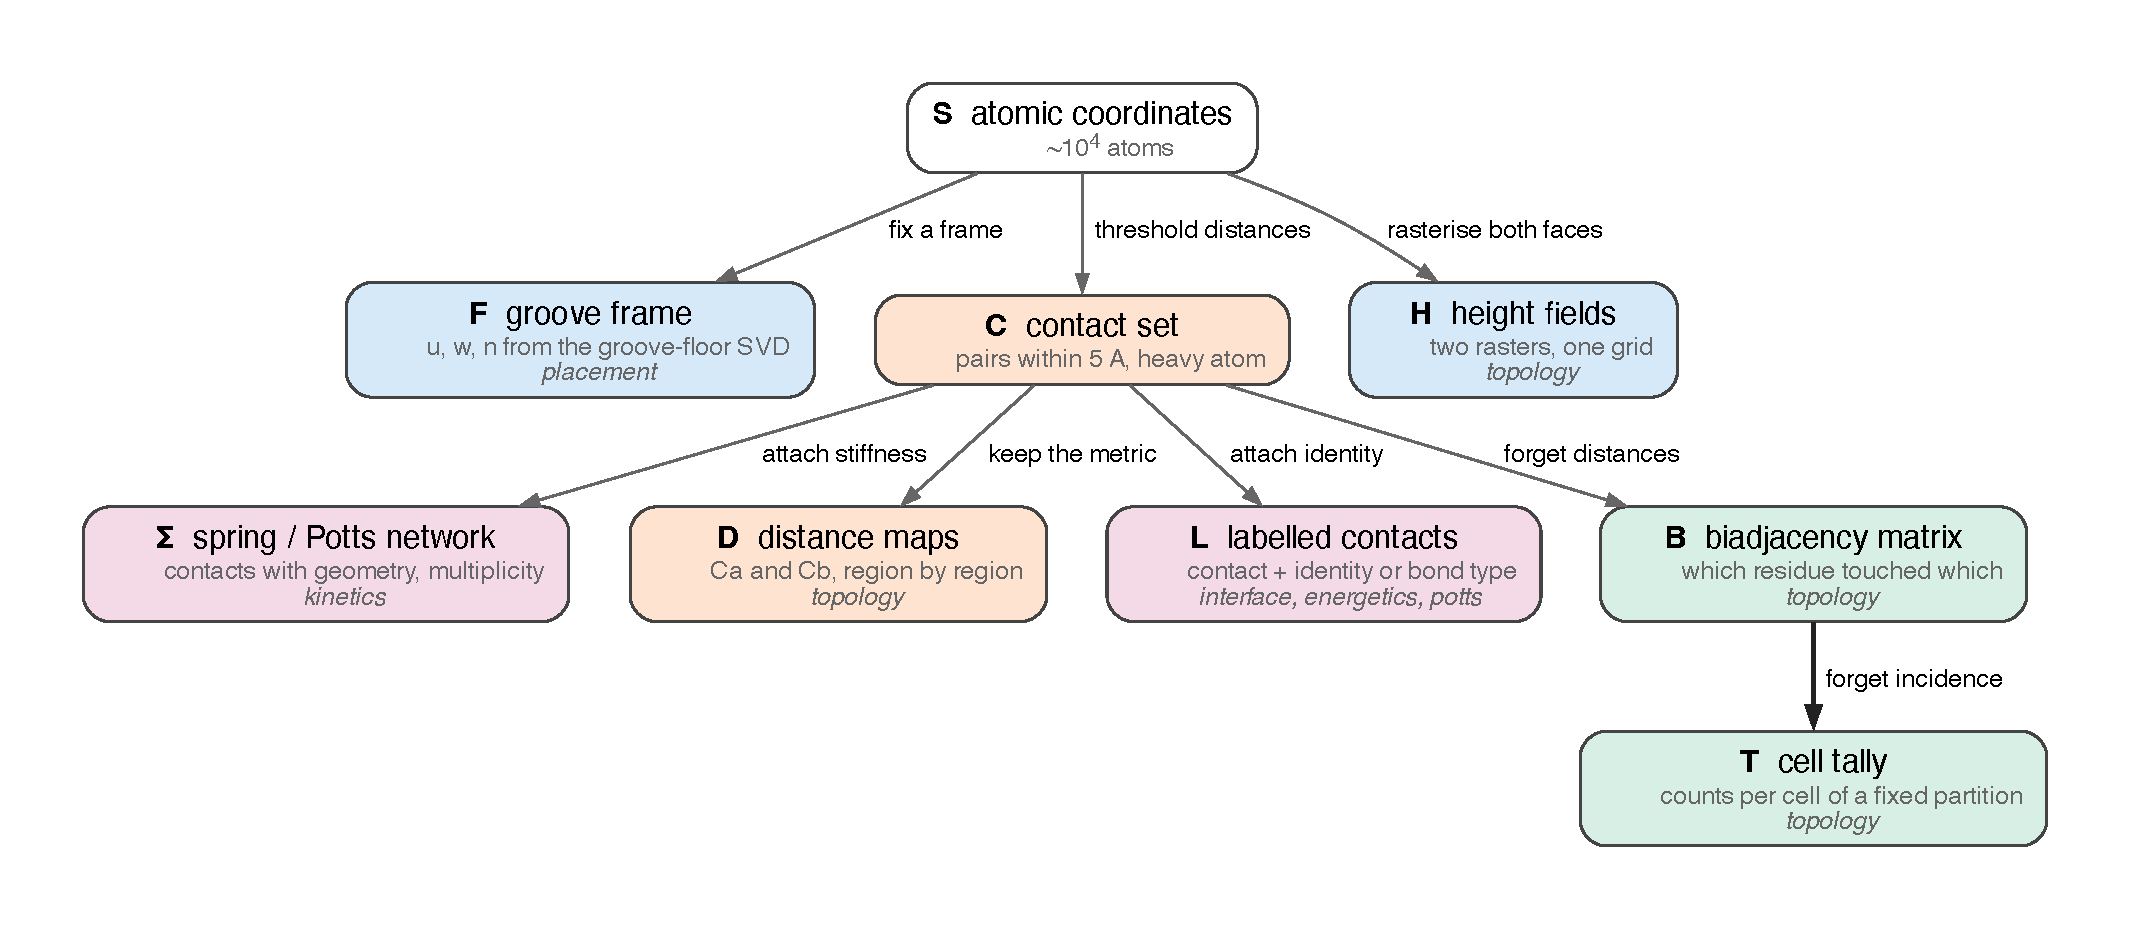
\includegraphics[width=0.92\textwidth]{generated/reduction.pdf}
\caption{The reduction chain. Each arrow discards information; the bold arrow
$\obj{B} \twoheadrightarrow \obj{T}$ is the one that matters most, because it is a quotient and
therefore orders the redundancy structure of \cref{sec:quotient}. The italic line in each node
names the family that reads that object; \emph{topology} appears in four, which is why it is the
largest family and the least coherent one.}
\label{fig:reduction}
\end{figure}

\begin{description}
\item[\obj{S}, the coordinates.] Around $10^4$ heavy atoms with chain, residue and region markup.
  Everything derives from here; no descriptor reads it directly.
\item[\obj{F}, the groove frame.] An orthonormal triple $(\hat u, \hat w, \hat n)$ obtained from the
  singular value decomposition of the MHC groove-floor C$\alpha$ coordinates, with the signs fixed
  by the peptide's N$\to$C direction and by which side the receptor sits on. \obj{F} is refit from
  every structure, which is what makes the placement family comparable across inputs.
\item[\obj{C}, the contact set.] Ordered pairs $(i,j)$ of residues whose closest heavy atoms lie
  within $5$~\AA. This is the single free parameter almost everything downstream inherits.
\item[\obj{D}, the distance maps.] The C$\alpha$ and C$\beta$ matrices between two labelled regions.
  \obj{D} keeps the metric and forgets the atoms.
\item[\obj{L}, the labelled contacts.] \obj{C} with residue identity, or with a bond type
  (salt bridge, hydrogen bond, aromatic, hydrophobic) attached. \obj{L} keeps chemistry and forgets
  geometry beyond the threshold.
\item[\obj{B}, the biadjacency matrix.] $B \in \{0,1\}^{m \times n}$ with the engaged CDR-loop
  residues as rows and the pMHC residues they touch as columns. \obj{B} keeps \emph{who touched
  whom} and forgets how far apart they were.
\item[\obj{T}, the cell tally.] Contact counts per cell of a fixed partition --- the twelve cells of
  six CDR loops $\times$ \{peptide, MHC\}, or the twenty-four that split the peptide into three
  bands. \obj{T} keeps how many and forgets which.
\item[\obj{H}, the height fields.] Two rasters $h_{\mathrm{pMHC}}(x,y)$ and $h_{\mathrm{TCR}}(x,y)$
  on one shared grid in the $\obj{F}$ plane, with per-cell charge and hydropathy painted on.
\item[$\Sigma$, the network.] \obj{C} with a stiffness or a Potts site attached to each pair: a
  spring network in the mechanical case, a set of occupiable sites in the Potts case.
\end{description}

\subsection{The quotient, and what it predicts}
\label{sec:quotient}

$\obj{B} \twoheadrightarrow \obj{T}$ is a quotient map: the tally is a function of the biadjacency
matrix, and many biadjacency matrices give the same tally. Every functional of \obj{T} is therefore
a functional of \obj{B}, and the converse fails. Two consequences follow without any measurement.

\begin{enumerate}
\item A \obj{T}-descriptor can be exactly determined by \obj{B}-descriptors, but no
  \obj{B}-descriptor can be exactly determined by \obj{T}-descriptors alone. Redundancy runs
  \emph{down} the chain, never up it.
\item The parameter-free replacements are the ones further \emph{up}. \dsc{g\_comp\_frac} counts
  components of the contact graph itself; \dsc{fp\_b0\_r7} counts components of a C$\alpha$ flag
  complex at an arbitrary $7$~\AA. The first reads \obj{B} and needs no radius; the second reads
  \obj{C} again with a second threshold on top of the first. When both survive a redundancy screen
  they are measuring different things; when only one does, the chain says which to prefer.
\end{enumerate}

\Cref{fig:quotient} draws the step for a small footprint.

\begin{figure}[t]
\centering
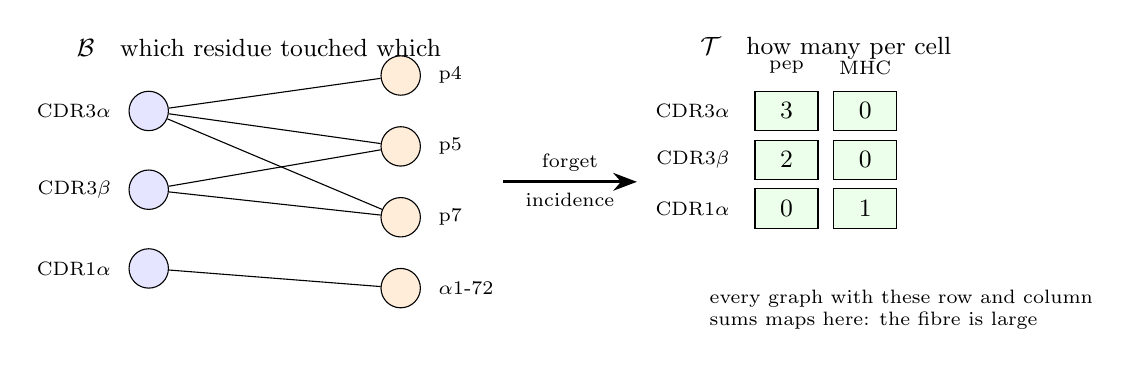
\begin{tikzpicture}[font=\small, node distance=3mm]
% --- left: the bipartite graph B
\node at (-0.2,3.1) {\textbf{\obj{B}} \ \ which residue touched which};
\foreach \i/\lab in {0/{CDR3$\alpha$},1/{CDR3$\beta$},2/{CDR1$\alpha$}}
  \node[circle,draw,fill=blue!10,inner sep=1.6pt,minimum size=5mm] (l\i) at (-1.6, 2.3-1.0*\i) {};
\foreach \i/\lab in {0/{CDR3$\alpha$},1/{CDR3$\beta$},2/{CDR1$\alpha$}}
  \node[left=1mm of l\i, font=\scriptsize] {\lab};
\foreach \j in {0,1,2,3}
  \node[circle,draw,fill=orange!15,inner sep=1.6pt,minimum size=5mm] (r\j) at (1.6, 2.75-0.9*\j) {};
\foreach \j/\lab in {0/{p4},1/{p5},2/{p7},3/{$\alpha$1-72}}
  \node[right=1mm of r\j, font=\scriptsize] {\lab};
\draw (l0)--(r0); \draw (l0)--(r1); \draw (l1)--(r1); \draw (l1)--(r2);
\draw (l2)--(r3); \draw (l0)--(r2);
% --- the arrow
\draw[-{Stealth[length=3mm]},very thick] (2.9,1.4) -- node[above,font=\scriptsize]{forget}
  node[below,font=\scriptsize]{incidence} (4.6,1.4);
% --- right: the tally T
\node at (7.0,3.1) {\textbf{\obj{T}} \ \ how many per cell};
\foreach \r/\lab in {0/{CDR3$\alpha$},1/{CDR3$\beta$},2/{CDR1$\alpha$}}
  \node[font=\scriptsize,anchor=east] at (5.9, 2.3-0.62*\r) {\lab};
\node[font=\scriptsize] at (6.5,2.85) {pep}; \node[font=\scriptsize] at (7.5,2.85) {MHC};
\foreach \r/\a/\b in {0/3/0, 1/2/0, 2/0/1} {
  \node[draw,fill=green!8,minimum width=8mm,minimum height=5mm] at (6.5, 2.3-0.62*\r) {\a};
  \node[draw,fill=green!8,minimum width=8mm,minimum height=5mm] at (7.5, 2.3-0.62*\r) {\b};
}
\node[font=\scriptsize,align=left,anchor=north west] at (5.4,0.15)
  {every graph with these row and column\\sums maps here: the fibre is large};
\end{tikzpicture}
\caption{The quotient $\obj{B} \twoheadrightarrow \obj{T}$ on a six-contact footprint. The tally
retains the row sums of the biadjacency matrix within each target block and discards which pMHC
residue each contact reached, so \dsc{g\_loop\_overlap} --- do the loops crowd onto the same
residues --- has no expression in \obj{T} at all.}
\label{fig:quotient}
\end{figure}

% =================================================================================================
\section{The operators}
\label{sec:operators}

\Cref{tab:operators} is the whole catalogue by what is applied rather than by what produced it.
Nine operators suffice, and two of them --- counts and frame coordinates --- need no derivation,
being the raw readings of \obj{L} and \obj{F} respectively. The remaining seven are derived below.

\begin{table}[t]
\centering
% GENERATED by scripts/gen_appendix.py -- do not edit.
\begin{tabular}{@{}llr@{}}
\toprule
operator & object read & descriptors \\
\midrule
count or share & $\mathcal{C}$, $\mathcal{L}$ & \textbf{49} \\
frame coordinate & $\mathcal{F}$ & 31 \\
field moment & $\mathcal{H}$, $\mathcal{D}$ & 19 \\
Hill number & $\mathcal{T}$, $\mathcal{B}$, spectra & 19 \\
potential sum & $\mathcal{L}$ & 19 \\
homology invariant & $\mathcal{B}$, $\mathcal{C}$ & 10 \\
spectral invariant & $\mathcal{B}$, $\mathcal{D}$, $\Sigma$ & 9 \\
correlation & $\mathcal{H}$, $\mathcal{D}$, $\mathcal{B}$ & 6 \\
mechanical work & $\Sigma$ & 2 \\
\midrule
total & & 164 \\
\bottomrule
\end{tabular}

\caption{The \nDesc\ descriptors by operator. Counts and shares dominate because the interface and
kinetics families are largely tallies; the interesting structure is in the smaller rows.}
\label{tab:operators}
\end{table}

% -------------------------------------------------------------------------------------------------
\subsection{Hill numbers: \nOpHill\ descriptors, one formula}
\label{sec:hill}

This is the largest unification in the catalogue and the one worth stating first. Let $p$ be a
probability vector on $k$ categories, $p_i \ge 0$, $\sum_i p_i = 1$. The \emph{Hill number of order
$q$} \cite{Hill1973,Jost2006} is the effective number of categories,
%
\begin{equation}
D_q(p) \;=\; \Big( \sum_{i \,:\, p_i > 0} p_i^{\,q} \Big)^{1/(1-q)},
\qquad
D_1(p) \;=\; \exp\Big( - \sum_i p_i \ln p_i \Big),
\label{eq:hill}
\end{equation}
%
where $D_1$ is the $q \to 1$ limit. Three orders are used: $D_0$ is the richness, the count of
occupied categories; $D_1$ is the exponentiated Shannon entropy; $D_2 = 1/\sum_i p_i^2$ is the
reciprocal of Simpson's concentration, and discounts weakly populated categories. All three are in
units of \emph{categories}, which is what makes them comparable across partitions of different
size, and each is bounded by $k$.

Four standard quantities are reparametrisations of \cref{eq:hill}, not separate ideas:

\begin{align}
\text{normalised Shannon entropy} && H &= \ln D_1 / \ln k, \label{eq:shannon}\\
\text{Pielou evenness} && J &= \ln D_1 / \ln D_0, \label{eq:pielou}\\
\text{participation ratio} && \mathrm{PR} &= D_2 / k, \label{eq:pr}\\
\text{Gini--Simpson index} && G &= 1 - 1/D_2. \label{eq:gini}
\end{align}

\Cref{eq:pielou} explains the \texttt{STATUS} entry that \dsc{J\_cell} is determined: it is
$H_{\mathrm{cell}} \ln 12 / \ln S_{\mathrm{cell}}$, a ratio of two shipped columns. \Cref{eq:pr} and
\cref{eq:gini} are the two that are \emph{not} yet recorded in \texttt{STATUS} and follow from the
algebra alone.

\Cref{tab:hill} instantiates the formula. Read a row as: take this probability vector, apply
\cref{eq:hill} at this order, then apply this normalisation.

\begin{table}[t]
\centering\small
\begin{tabular}{@{}llcl@{}}
\toprule
descriptor & $p$ is over & $q$ & normalisation \\
\midrule
\dsc{S\_cell}            & the 12 cells, contact shares                    & 0 & none \\
\dsc{D1\_cell}           & the 12 cells                                    & 1 & none \\
\dsc{H\_cell}            & the 12 cells                                    & 1 & $\ln D_1 / \ln 12$ \\
\dsc{D2\_cell}           & the 12 cells                                    & 2 & none \\
\dsc{J\_cell}            & the 12 cells                                    & 1 & $\ln D_1 / \ln D_0$ \\
\addlinespace
\dsc{H\_loop}            & the 6 CDR loops, contact shares                 & 1 & $\ln D_1 / \ln 6$ \\
\dsc{D2\_loop}           & the 6 CDR loops                                 & 2 & none \\
\dsc{D2\_pep24}          & the 24 cells (peptide split in three bands)     & 2 & none \\
\addlinespace
\dsc{pep\_cov\_even}     & $L$ peptide positions, accessibility-discounted & 1 & $\ln D_1 / \ln L$ \\
\dsc{pep\_cov\_d2n}      & the same                                        & 2 & $D_2 / L$ \\
\addlinespace
\dsc{g\_even\_tcr}       & degrees of the $m$ engaged TCR residues         & 1 & $\ln D_1 / \ln m$ \\
\dsc{g\_even\_pmhc}      & degrees of the $n$ engaged pMHC residues        & 1 & $\ln D_1 / \ln n$ \\
\dsc{g\_loop\_even}      & distinct partners per CDR loop                  & 1 & $\ln D_1 / \ln 6$ \\
\dsc{degree\_evenness\_tp} & TCR-side degrees, TCR:peptide only            & 2 & $D_2 / m$ \\
\addlinespace
\dsc{m\_erank\_tp}       & singular values of $K_{\mathrm{tp}}$, normalised & 2 & $D_2 / \min(L,M)$ \\
\dsc{m\_erank\_tm}       & singular values of $K_{\mathrm{tm}}$, normalised & 2 & $D_2 / \min(L,M)$ \\
\dsc{h0\_pers\_ent}      & minimum-spanning-tree edge lengths              & 1 & $\ln D_1 / \ln(n{-}1)$ \\
\addlinespace
\dsc{partcoef\_tcr}      & per-residue shares over \{peptide, MHC\}        & 2 & $\mathrm{mean}_i(1 - 1/D_2)$ \\
\dsc{partcoef\_pmhc}     & per-residue shares over the 6 CDR loops         & 2 & $\mathrm{mean}_i(1 - 1/D_2)$ \\
\bottomrule
\end{tabular}
\caption{\nOpHill\ descriptors across four families as one formula: seven probability vectors,
three orders, five normalisations. \dsc{S\_cell} through \dsc{D2\_pep24} read \obj{T};
\dsc{g\_even\_*} through \dsc{partcoef\_*} read \obj{B}; the \dsc{m\_erank\_*} pair reads a spectrum
of \obj{D}; \dsc{h0\_pers\_ent} reads a barcode of \obj{C}.}
\label{tab:hill}
\end{table}

\paragraph{Three identities worth naming.}
Each follows from \cref{eq:hill} and can be checked in a line.

\begin{enumerate}
\item \emph{Di Paola's participation coefficient is Gini--Simpson.} The published definition
  \cite{DiPaola2015} is $P_i = 1 - \sum_s (k_{si}/k_i)^2$ over modules $s$, with $k_{si}$ residue
  $i$'s edge count into module $s$. Writing $p_s = k_{si}/k_i$ gives $\sum_s p_s^2 = 1/D_2(p)$, so
  $P_i = 1 - 1/D_2$ exactly --- \cref{eq:gini}. It is a diversity of order 2 on a per-residue
  module profile, which places it in \cref{tab:hill} rather than beside it.
\item \emph{Effective rank and cell entropy are the same operator.} \dsc{m\_erank\_tp} applies
  \cref{eq:hill} to the normalised singular-value spectrum of a proximity kernel;
  \dsc{D2\_cell} applies it to a contact tally. They are not independent descriptor families and
  should not be presented as such --- what differs is the input, not the measure.
\item \emph{The shipped effective rank is order 2, not order 1.} Roy and Vetterli's Definition 1
  \cite{RoyVetterli2007} is $\mathrm{erank}(A) = \exp\{H(p_1,\dots,p_Q)\}$ with
  $p_k = \sigma_k / \|\sigma\|_1$, $Q = \min\{M,N\}$ and $H$ the Shannon entropy --- that is
  exactly $D_1$ of the normalised spectrum.
  The shipped \dsc{m\_erank\_*} computes $(\sum_a s_a)^2 / \sum_a s_a^2$, which is $D_2$ --- the
  participation ratio, as the implementing function's own docstring says. Both are legitimate
  effective ranks and $D_2 \le D_1$ always; the name in the descriptor table points at the
  literature quantity while the code computes the order-2 sibling. Anyone comparing our column
  against a published effective rank must use $q = 2$.
\end{enumerate}

\paragraph{Why several orders ship at once.} $D_1$ and $D_2$ rank differently. $D_1$ weights
categories by their share; $D_2$ weights by the square, so a footprint with one dominant cell and a
long tail of singletons scores much lower at $q=2$ than at $q=1$. Keeping both is the deliberate
choice the library has made since the coverage block was written, and it is why \dsc{D2\_pep24}
rather than \dsc{H\_cell} carries the shape channel.

% -------------------------------------------------------------------------------------------------
\subsection{Field moments, and the gap resolved by sign}
\label{sec:moments}

The second operator takes moments of a scalar field defined on a shared index --- grid cells for the
surface block, contacting residue pairs for the map block. \nOpMoment\ descriptors, of which nine
read one field: the gap between the two faces.

\paragraph{The two faces and their difference.} \obj{H} carries two height fields on \emph{one}
grid: $h_{\mathrm{pMHC}}(x,y)$, the highest pMHC surface point in cell $(x,y)$, and
$h_{\mathrm{TCR}}(x,y)$, the lowest receptor point in the same cell, both in the groove frame
$(\hat u, \hat w, \hat n)$ of \cref{sec:frame} with $\hat n$ pointing at the receptor. Because they
share a grid, the space between them is a subtraction rather than a new geometric construction:
%
\begin{equation}
\mathrm{gap}(x,y) \;=\; h_{\mathrm{TCR}}(x,y) - h_{\mathrm{pMHC}}(x,y) \quad [\text{\AA}].
\label{eq:gap}
\end{equation}
%
A cell enters the comparison when both faces reach it and $|\mathrm{gap}| \le 10$~\AA, cropped to a
$\pm 12$~\AA\ window about the groove centre; the retained set is $R$ with $|R| =$ \dsc{sc\_cells}
and area element $\delta A = 0.977$~\AA$^2$.

\paragraph{The sign is not the one intuition suggests.} A gap is naturally imagined as a void, so
$\mathrm{gap} > 0$. Measured over the crystal reference set it is predominantly negative: the
receptor's lowest point in a cell lies \emph{below} the groove's highest point in the same cell,
because the two faces interdigitate rather than stack. Over 371 of the 374 crystals the mean
interdigitated fraction is $0.750$ (s.d.\ $0.096$) and the mean gap $-1.14$~\AA. Pooling the two
signs into one mean therefore cancels the physics, which is why the field is reported three ways
(\cref{fig:gap}).

\begin{figure}[t]
\centering
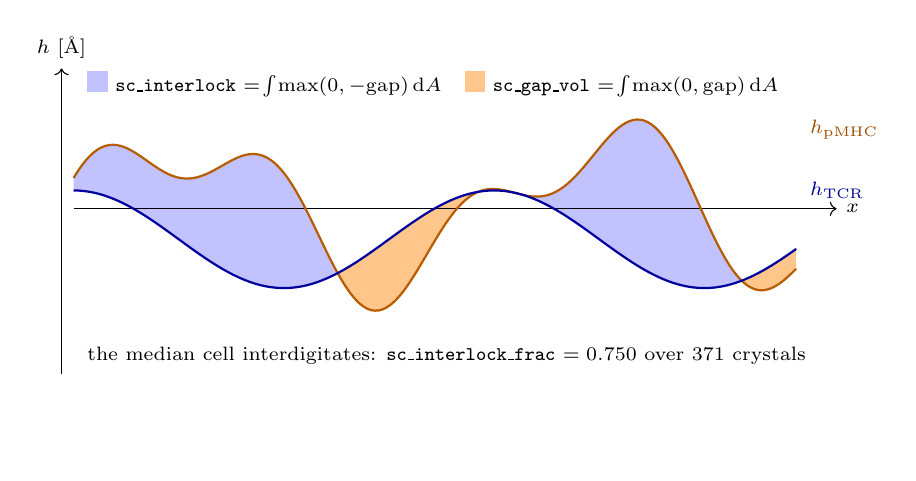
\begin{tikzpicture}[font=\small,xscale=1.02,yscale=1.55]
% h_pMHC = 0.55 sin(1.2x) + 0.30 sin(2.7x + 1);  h_TCR = 0.40 sin(1.2x + pi/2) - 0.25.
% Chosen so the interdigitated share is 0.715 -- close to the measured 0.750 -- with the void
% patches deep enough to see. A drawing where the receptor never rises above the groove would
% claim 1.0 and misstate the result.
\def\hpmhc{0.55*sin(68.755*\x) + 0.30*sin(154.70*\x + 57.3)}
\def\htcr{0.40*sin(68.755*\x + 90) - 0.25}
% shade: interlock, TCR below pMHC
\begin{scope}
\clip plot[smooth,domain=0:9,samples=200] (\x, {\hpmhc}) -- (9,-2) -- (0,-2) -- cycle;
\fill[blue!24] plot[smooth,domain=0:9,samples=200] (\x, {\htcr}) -- (9,2) -- (0,2) -- cycle;
\end{scope}
% shade: void, TCR above pMHC
\begin{scope}
\clip plot[smooth,domain=0:9,samples=200] (\x, {\htcr}) -- (9,-2) -- (0,-2) -- cycle;
\fill[orange!45] plot[smooth,domain=0:9,samples=200] (\x, {\hpmhc}) -- (9,2) -- (0,2) -- cycle;
\end{scope}
\draw[->] (-0.15,-1.35) -- (-0.15,1.15) node[above,font=\scriptsize] {$h$ [\AA]};
\draw[->] (0,0) -- (9.5,0) node[right,font=\scriptsize] {$x$};
\draw[thick,orange!72!black] plot[smooth,domain=0:9,samples=200] (\x, {\hpmhc});
\draw[thick,blue!62!black]   plot[smooth,domain=0:9,samples=200] (\x, {\htcr});
\node[orange!62!black,font=\scriptsize,anchor=west] at (9.05,0.65) {$h_{\mathrm{pMHC}}$};
\node[blue!58!black,font=\scriptsize,anchor=west]   at (9.05,0.15) {$h_{\mathrm{TCR}}$};
\node[font=\scriptsize,anchor=west] at (0.05,1.02)
  {\tikz\fill[blue!24](0,0)rectangle(2.6mm,2.6mm);\ \dsc{sc\_interlock} $=\!\int\!\max(0,-\mathrm{gap})\,\mathrm{d}A$};
\node[font=\scriptsize,anchor=west] at (4.75,1.02)
  {\tikz\fill[orange!45](0,0)rectangle(2.6mm,2.6mm);\ \dsc{sc\_gap\_vol} $=\!\int\!\max(0,\mathrm{gap})\,\mathrm{d}A$};
\node[font=\scriptsize,anchor=west] at (0.05,-1.20)
  {the median cell interdigitates: \dsc{sc\_interlock\_frac} $= 0.750$ over 371 crystals};
\end{tikzpicture}
\caption{The gap field in cross-section. Blue is interdigitated volume, orange is void; the two are
integrated separately because a mean over the retained cells cancels them against each other. On a
real interface the blue area is the larger, by roughly $1{,}004$ against $373$~\AA$^3$.}
\label{fig:gap}
\end{figure}

The nine gap descriptors are then
%
\begin{align}
\text{pooled} &&
\dsc{sc\_gap\_mean} &= \frac{1}{|R|}\sum_{R} \mathrm{gap}, &
\dsc{sc\_gap\_sd} &= \mathrm{sd}_{R}(\mathrm{gap}), \\
\text{integrated} &&
\dsc{sc\_gap\_vol} &= \delta A \!\! \sum_{R} \max(0, \mathrm{gap}), &
\dsc{sc\_interlock} &= \delta A \!\! \sum_{R} \max(0, -\mathrm{gap}), \\
&& \dsc{sc\_gap\_index} &= \dsc{sc\_gap\_vol} / (|R|\,\delta A), \\
\text{by sign} &&
\phi &= \tfrac{1}{|R|}\big|\{\mathrm{gap} < 0\}\big|, &
\dsc{sc\_gap\_depth} &= -\overline{\mathrm{gap}}\big|_{\mathrm{gap}<0}, \\
&& \dsc{sc\_gap\_height} &= \overline{\mathrm{gap}}\big|_{\mathrm{gap}>0}, &
\dsc{sc\_gap\_asym} &= \frac{V_{+} - V_{-}}{V_{+} + V_{-}},
\end{align}
%
with $\phi =$ \dsc{sc\_interlock\_frac}, $V_+ =$ \dsc{sc\_gap\_vol} and $V_- =$ \dsc{sc\_interlock}.
The decomposition is exact and is asserted by a unit test rather than assumed:
%
\begin{equation}
\dsc{sc\_gap\_mean} \;=\; (1-\phi)\cdot\dsc{sc\_gap\_height} \;-\; \phi \cdot \dsc{sc\_gap\_depth}.
\label{eq:gapdecomp}
\end{equation}
%
\Cref{eq:gapdecomp} is the reason the pooled mean is kept alongside the sign-resolved triple: it is
their $\phi$-weighted combination, so it is redundant with them by construction and is retained only
as the familiar summary.

\paragraph{Attribution.} \dsc{sc\_gap\_index} is the intensive form of the gap channel and takes
the shape of Jones and Thornton's gap volume index \cite{JonesThornton1996}, but ours divides by the
retained contact area of the raster rather than by an interface accessible surface area, and the
underlying field is a raster subtraction rather than a Voronoi gap volume. The channel is theirs;
the quantity is not, and should not be cited as if it were.

\paragraph{The other field moments.} \dsc{sc\_dh}, \dsc{sc\_dcharge} and \dsc{sc\_dphobic} are mean
absolute per-cell differences of the height, charge and Kyte--Doolittle fields;
\dsc{sc\_charge\_prod} and \dsc{sc\_phobic\_prod} their mean per-cell products.
\dsc{m\_face\_tp} and \dsc{m\_face\_tm} take a moment on a different index --- contacting residue
pairs rather than grid cells:
%
\begin{equation}
\dsc{m\_face} \;=\; \frac{1}{|C|}\sum_{(i,j) \in C}
\big( \| \mathrm{C}\alpha_i - \mathrm{C}\alpha_j \| - \| \mathrm{C}\beta_i - \mathrm{C}\beta_j \| \big),
\label{eq:face}
\end{equation}
%
positive when the side chains lean towards each other and negative when the backbones are the close
part and the side chains point away. \Cref{eq:face} is the one quantity in the catalogue that
C$\alpha$ coordinates alone cannot express, which is its reason for existing.

% -------------------------------------------------------------------------------------------------
\subsection{Correlation over a shared index}

\nOpCorrelation\ descriptors are a correlation coefficient between two vectors indexed by the same
set. The operator is trivial; what varies is the index and the pair of fields, and the sign
convention differs between them, which is the only thing a reader has to remember.

\begin{center}\small
\begin{tabular}{@{}lp{0.24\textwidth}p{0.26\textwidth}l@{}}
\toprule
descriptor & index & fields & complementary when \\
\midrule
\dsc{sc\_shape}   & retained grid cells & the two height fields    & $r > 0$ \\
\dsc{sc\_charge}  & retained grid cells & the two charge fields    & $r < 0$ \\
\dsc{sc\_phobic}  & retained grid cells & the two hydropathy fields& $r > 0$ \\
\dsc{ca\_cb\_agreement\_tp} & TCR:peptide shell pairs & C$\alpha$ and C$\beta$ maps & $\rho$ high \\
\dsc{ca\_cb\_agreement\_tm} & TCR:MHC shell pairs     & C$\alpha$ and C$\beta$ maps & $\rho$ high \\
\dsc{g\_assort}   & the $E$ contacts    & degrees at the two ends  & --- \\
\bottomrule
\end{tabular}
\end{center}

\dsc{sc\_charge} inverts because charge complementarity is plus meeting minus, whereas shape and
apolar complementarity are like meeting like. \dsc{sc\_shape} is Lawrence and Colman's shape
complementarity idea \cite{LawrenceColman1993} carried onto a raster: their $S_c$ is a median over
dot-surface points of $(\mathbf{n}_A \!\cdot\! \mathbf{n}'_A)\exp(-w d^2)$ after trimming a
peripheral band, and ours is a Pearson correlation of two height fields. The construction differs;
the channel is the same one, and the resemblance should be stated that way rather than as a
reimplementation.

\dsc{g\_assort} is degree assortativity \cite{Newman2002}, correlating the degrees at the two ends
of each edge. It is left undefined rather than zero when either side has constant degree: there is
no correlation to measure, which is not the same as measuring no correlation. Assortativity is
partly determined by the degree distribution itself \cite{BaglerSinha2007}, so it is not independent
of \dsc{g\_even\_tcr} and \dsc{g\_even\_pmhc} and should be read beside them.

% -------------------------------------------------------------------------------------------------
\subsection{Spectral invariants}

\nOpSpectral\ descriptors are eigenvalues or singular values of an operator built from geometry.
Three constructions.

\paragraph{The normalised Laplacian.} On the largest component of the bipartite contact graph, with
$A$ the adjacency matrix and $D$ the degree matrix,
%
\begin{equation}
\mathcal{L} \;=\; I - D^{-1/2} A D^{-1/2}, \qquad
\dsc{g\_alg\_conn} \;=\; \lambda_2(\mathcal{L}) \in [0,2],
\label{eq:laplacian}
\end{equation}
%
the algebraic connectivity \cite{Fiedler1973}: near zero when the footprint is about to fall into
two patches, so it is the continuous form of the Betti-0 count of \cref{sec:homology}. The
normalisation matters. The combinatorial Laplacian's $\lambda_2$ scales with degree and would track
interface size; \cref{eq:laplacian} is bounded. One caution follows from the same normalisation:
$\lambda_{\max}(\mathcal{L}) = 2$ identically for \emph{any} bipartite graph, and our contact graph
is bipartite by construction, so $\lambda_{\max}$ carries no information here and must never be
added as a descriptor.

\paragraph{The proximity kernel.} For two labelled regions with C$\alpha$ distance map
$D \in \mathbb{R}^{L \times M}$, the Gaussian proximity kernel and its singular values
$s_1 \ge s_2 \ge \cdots$ are
%
\begin{equation}
K \;=\; \exp\!\big( -D^{\odot 2} / 2\sigma^2 \big), \qquad \sigma = 5\ \text{\AA},
\qquad
\dsc{m\_gap} \;=\; s_2/s_1 .
\label{eq:kernel}
\end{equation}
%
$\sigma$ is the contact criterion's own $5$~\AA, so the binary contact map is this kernel's
$\sigma \to 0$ limit rather than an independent parameter. The entries of $D$ cannot be compared
across a 9-mer and a 15-mer, or across CDR3 loops of different length; its singular values can,
which is the whole point of the construction. $s_2/s_1$ is near zero when the approach is separable
--- a rank-one $K$ means a loop profile times a peptide profile, a receptor leaning on a surface
rather than pairing specific residues with it. The corresponding $D_2$ of the same spectrum is
\dsc{m\_erank}, \cref{sec:hill}.

\paragraph{The stiffness tensor.} Each inter-body residue contact is a Hookean spring anchored at
the two C$\alpha$ atoms, with stiffness $k_i$ from heavy-atom-pair multiplicity divided by squared
distance and unit direction $\hat u_i$. The interface linear-response stiffness is
%
\begin{equation}
K \;=\; \sum_i k_i \, \hat u_i \otimes \hat u_i \in \mathbb{R}^{3\times 3},
\qquad
\dsc{S\_tot} = \operatorname{tr} K, \quad
\dsc{lam\_max}, \dsc{lam\_min} = \lambda_{\max,\min}(K).
\label{eq:stiffness}
\end{equation}
%
\dsc{K\_tens} is the component along the docking axis, \dsc{K\_shear} $= \operatorname{tr} K -
\dsc{K\_tens}$ the in-plane remainder and \dsc{aniso} their ratio; the last three are exactly
determined by the first two and are flagged as such. No potential enters \cref{eq:stiffness} --- it
is geometry and multiplicity only, which is what makes \dsc{rupture\_work} an off-rate proxy
independent of the energy channel it is compared against.

% -------------------------------------------------------------------------------------------------
\subsection{Homology invariants}
\label{sec:homology}

\nOpHomology\ descriptors count connected components and independent cycles, on two different
complexes, and the difference between the two complexes is the whole story.

\paragraph{The C$\alpha$ flag complex.} Take the contacted pMHC C$\alpha$ atoms, join any pair
within $r$, and build the flag (clique) complex. \dsc{fp\_b0\_r7} and \dsc{fp\_b1\_r7} are its Betti
numbers at $r = 7$~\AA, \dsc{fp\_chi\_r7} $= b_0 - b_1$ the Euler characteristic --- determined, and
flagged --- and \dsc{fp\_b0\_frac\_r7} is $b_0$ per contacted residue, the size-free form. The same
four at $r = 8$~\AA.

\paragraph{The contact graph itself.} \dsc{g\_comp\_frac} $= C/V$ and
%
\begin{equation}
\dsc{g\_cyclo\_frac} \;=\; \frac{E - V + C}{E},
\label{eq:cyclo}
\end{equation}
%
with $E$ contacts, $V = m+n$ residues and $C$ components. The numerator of \cref{eq:cyclo} is the
cyclomatic number, which for a graph is the first Betti number; dividing by $E$ is what makes it
size-free, and the footprint module rejects the raw form precisely because with of order thirty
contacts among of order thirty residues it is dominated by $E$ and simply tracks interface size.

\paragraph{Which to prefer.} The flag-complex pair introduces a \emph{second} threshold on top of
the $5$~\AA\ contact criterion, and $7$ and $8$~\AA\ are not derived from anything. The contact
graph pair introduces none. By the ordering of \cref{sec:quotient} the parameter-free form is the
one to prefer where both are informative --- which is a statement about parsimony, not about
measured performance; the flag-complex columns carry benchmark numbers and are not being retired
here.

\paragraph{Persistence entropy.} \dsc{h0\_pers\_ent} belongs to this section by provenance and to
\cref{sec:hill} by formula. The $H_0$ barcode's death times are exactly the minimum spanning tree's
edge lengths, so no filtration library is needed: build the tree, normalise the edge lengths to a
probability vector, take \cref{eq:shannon}. It is scale-free by construction.

% -------------------------------------------------------------------------------------------------
\subsection{Potential sums}
\label{sec:potential}

\nOpPotential\ descriptors sum a pair potential over a contact set, or take a difference of two such
sums. The Hamiltonian is
%
\begin{equation}
\Phi \;=\; c_{\mathrm{TP}}\,\Phi_{\mathrm{TCR:pep}}
       \;+\; c_{\mathrm{TM}}\,\Phi_{\mathrm{TCR:MHC}}
       \;+\; c_{\mathrm{PM}}\,\Phi_{\mathrm{pep:MHC}},
\qquad
\Phi_I \;=\; \sum_{(i,j) \in C_I} e_I(a_i, a_j),
\label{eq:phi}
\end{equation}
%
where $C_I$ is interface $I$'s contact set, $a_i$ the amino acid at residue $i$, and $e_I$ that
interface's potential --- TCRen2 for TCR:peptide, Miyazawa--Jernigan \cite{MiyazawaJernigan1996} for
the two presentation interfaces. The coefficients exist because the three interfaces are scored with
\emph{different potentials on different scales}; each term enters divided by that interface energy's
spread over the crystal reference set, $c_I = 1/\mathrm{sd}(\Phi_I)$. Lower $\Phi$ is more
favourable throughout.

\paragraph{What cancels.} Because no interface energy carries a within-chain term, varying the
peptide leaves $\Phi_{\mathrm{TCR:MHC}}$ untouched and varying the TCR leaves
$\Phi_{\mathrm{pep:MHC}}$ untouched --- exactly, not approximately, since a truncated side chain
moves no atom of the other two chains. This is why a peptide-ranking task reads
$\Delta\Phi_{\mathrm{TCR:pep}}$ and a receptor-ranking task does not read
$\Delta\Phi_{\mathrm{pep:MHC}}$ at all.

\paragraph{The reference difference.} $\Delta\Phi$ (written \dsc{dPhi\_*}) is the difference of
$\Phi$ against a reference \emph{sequence}, never a derivative:
$\Delta\Phi = \Phi(\text{sequence}) - \Phi(\text{reference})$. In the hard form the reference is
poly-alanine, one arbitrary sequence. In the smoothed form it is the free energy of the residue
\emph{background}, which is a distribution rather than a choice. Since $\Phi$ is a sum of
independent local fields over the varying positions,
%
\begin{equation}
\varphi_i(a) \;=\; \sum_{I} c_I \!\!\sum_{j \,:\, (i,j) \in C_I} \!\! e_I(a, y_j),
\label{eq:localfield}
\end{equation}
%
with $y$ the frozen partners, the partition function factorises exactly and the reference free
energy is available in closed form:
%
\begin{equation}
\Phi_{\mathrm{ref}} \;=\; -\frac{1}{\beta}\sum_i \log \sum_a p(a)\, e^{-\beta \varphi_i(a)},
\qquad
\Delta\Phi \;=\; \Phi(\text{observed}) - \Phi_{\mathrm{ref}},
\label{eq:softref}
\end{equation}
%
$p$ being the background composition over the twenty amino acids. The second cumulant of the same
log partition function is the variance descriptor,
%
\begin{equation}
\operatorname{Var}\Phi \;=\; \sum_i \operatorname{Var}_\beta[\varphi_i],
\qquad
\operatorname{Var}_\beta \ \text{under} \
\frac{p(a)e^{-\beta\varphi_i(a)}}{\sum_b p(b)e^{-\beta\varphi_i(b)}} .
\label{eq:varphi}
\end{equation}
%
\Cref{eq:varphi} asks how sharply a position's energy responds to residue identity at all: a
position whose twenty fields are equal contributes to neither $\Delta\Phi$ nor $\operatorname{Var}
\Phi$; one with a single strongly preferred residue contributes to both. It is a second cumulant,
not a difference of differences, and the catalogue carries no $\mathrm{d}\mathrm{d}$ quantity --- the
only one in the package is $\Delta\Delta G$, the change in binding free energy on mutation, which is
not a descriptor.

% -------------------------------------------------------------------------------------------------
\subsection{The Potts family}

Five descriptors read the same interface against a partition function rather than against a
reference sequence. The configuration is the contact map itself: sites $a$ are the residue pairs
that \emph{could} have contacted (C$\alpha$ within a radius) and $\sigma_a = 1$ iff a heavy-atom
contact formed. With one-body fields $\eta$ and couplings $A$ between neighbouring cells of the map,
%
\begin{equation}
E(\sigma) = -\sum_a \eta_a \sigma_a - \tfrac{1}{2}\sum_{a,b} A_{ab}\sigma_a\sigma_b,
\qquad
P(\sigma) = e^{-E(\sigma)}/Z .
\label{eq:potts}
\end{equation}
%
\dsc{neg\_energy} is $-E(\sigma^{\mathrm{obs}})$, \dsc{log\_z} is $\log Z$ over every contact map the
geometry admits --- the interface's \emph{capacity} --- and \dsc{log\_lik} is $\log P(\sigma^{\mathrm
{obs}})$, its \emph{typicality}. \dsc{psi} is \dsc{log\_lik} per available site, so interfaces of
different size compare. The three are not independent:
%
\begin{equation}
\dsc{neg\_energy} \;=\; \dsc{log\_z} + \dsc{log\_lik},
\label{eq:pottsid}
\end{equation}
%
directly from \cref{eq:potts}, and \cref{eq:pottsid} is the \texttt{STATUS} entry on
\dsc{neg\_energy}. Fitting is by penalised pseudolikelihood and needs no $Z$; scoring obtains $Z$ by
annealed importance sampling from the uncoupled model, whose partition function is exact.

% -------------------------------------------------------------------------------------------------
\subsection{Frame coordinates}
\label{sec:frame}

The \nOpFrame\ placement descriptors are the rigid-body pose and the two CDR3 loops expressed in the
groove frame. They are the only family that needs a frame at all, and the frame is refit from every
structure (\cref{fig:frame}).

\begin{figure}[t]
\centering
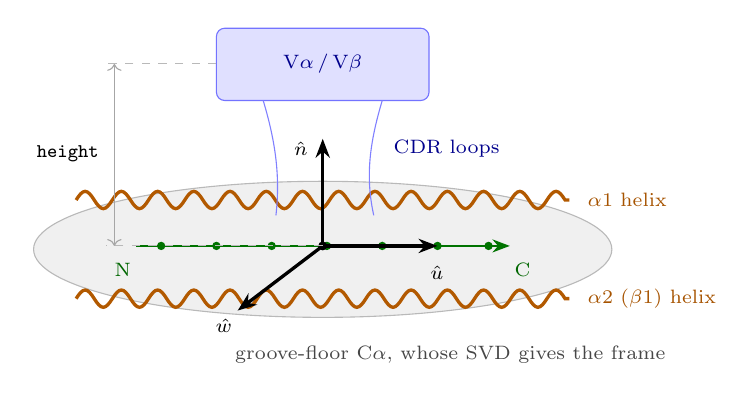
\begin{tikzpicture}[font=\small,scale=1.08]
% groove floor, and its label BELOW the ellipse -- the short-axis arrow used to strike through it
\draw[fill=gray!12,draw=gray!55] (0,0) ellipse (3.4 and 0.8);
\node[gray!55!black,font=\scriptsize,anchor=north] at (1.5,-1.02)
  {groove-floor C$\alpha$, whose SVD gives the frame};
% helices
\draw[very thick,orange!70!black,decorate,
      decoration={coil,aspect=0,segment length=4.6mm,amplitude=1.1mm}] (-2.9,0.58) -- (2.9,0.58);
\draw[very thick,orange!70!black,decorate,
      decoration={coil,aspect=0,segment length=4.6mm,amplitude=1.1mm}] (-2.9,-0.58) -- (2.9,-0.58);
\node[orange!65!black,font=\scriptsize,anchor=west] at (3.0,0.58) {$\alpha$1 helix};
\node[orange!65!black,font=\scriptsize,anchor=west] at (3.0,-0.58) {$\alpha$2 ($\beta$1) helix};
% peptide, N to C
\draw[thick,green!45!black,-{Stealth[length=2.2mm]}] (-2.2,0.04) -- (2.2,0.04);
\foreach \x in {-1.9,-1.25,-0.6,0.05,0.7,1.35,1.95} \fill[green!45!black] (\x,0.04) circle (1.4pt);
\node[green!40!black,font=\scriptsize] at (-2.35,-0.24) {N};
\node[green!40!black,font=\scriptsize] at (2.35,-0.24) {C};
% TCR body and the loops reaching down
\draw[fill=blue!12,draw=blue!55,rounded corners=3pt] (-1.25,1.75) rectangle (1.25,2.6);
\node[blue!55!black,font=\scriptsize] at (0,2.18) {V$\alpha$\,/\,V$\beta$};
\draw[blue!50] (-0.7,1.75) .. controls (-0.55,1.25) and (-0.5,0.85) .. (-0.55,0.40);
\draw[blue!50] (0.7,1.75)  .. controls (0.55,1.25) and (0.5,0.85)  .. (0.6,0.40);
\node[blue!55!black,font=\scriptsize,anchor=west] at (0.72,1.18) {CDR loops};
% the frame: u in plane, n up, w foreshortened down-LEFT into free space
\draw[-{Stealth[length=2.4mm]},very thick] (0,0.04) -- (1.35,0.04);
\node[font=\scriptsize,anchor=north west] at (1.15,-0.08) {$\hat u$};
\draw[-{Stealth[length=2.4mm]},very thick] (0,0.04) -- (0,1.30);
\node[font=\scriptsize,anchor=east] at (-0.06,1.18) {$\hat n$};
\draw[-{Stealth[length=2.4mm]},very thick] (0,0.04) -- (-1.00,-0.72);
\node[font=\scriptsize,anchor=north east] at (-0.95,-0.70) {$\hat w$};
\fill (0,0.04) circle (1.5pt);
% height, measured on the left where nothing else is
\draw[gray!55,dashed] (-1.25,2.18) -- (-2.55,2.18);
\draw[gray!55,dashed] (0,0.04) -- (-2.55,0.04);
\draw[<->,gray!70] (-2.45,0.04) -- (-2.45,2.18);
\node[font=\scriptsize,anchor=east] at (-2.52,1.12) {\dsc{height}};
\end{tikzpicture}
\caption{The groove frame. $\hat u$, $\hat w$ and $\hat n$ come from the singular value
decomposition of the groove-floor C$\alpha$ coordinates, with signs fixed by the peptide's N$\to$C
direction and by which side the receptor sits on. Every placement descriptor is a length, an angle
or a direction cosine in this frame, so all thirty-one are $SE(3)$-invariant despite reading a
frame.}
\label{fig:frame}
\end{figure}

Six of them are the rigid-body pose: \dsc{dock\_d} the stub-to-stub separation, \dsc{dock\_torsion}
the dihedral of the TCR about the MHC stub, and the four direction cosines \dsc{dock\_tcr\_uy},
\dsc{dock\_tcr\_uz}, \dsc{dock\_mhc\_uy}, \dsc{dock\_mhc\_uz}. Four more locate the CDR centroid:
\dsc{height} above the groove plane, \dsc{shift\_u} and \dsc{shift\_w} in plane, and
\dsc{offset} $= \sqrt{\dsc{shift\_u}^2 + \dsc{shift\_w}^2}$, which is determined by the two and
flagged. Twenty are the two CDR3 loops, each contributing a reach, three position cosines, three
axis cosines, an engagement depth and an extension.

\paragraph{The crossing angle, and one banned column.} \dsc{crossing\_signed} is the angle between
the V$\alpha \to$ V$\beta$ axis projected into the groove plane and the groove long axis, on
$[-180^\circ, 180^\circ)$; its \emph{sign} is the docking polarity, canonical or reversed, and
\dsc{crossing} $= |\dsc{crossing\_signed}|$ is determined by it. Polarity and angle are different
quantities and conflating them is a category error: docking polarity is stereotyped across complexes
whose crossing angles vary widely \cite{Feng2007}, and reversed-polarity receptors bind but cannot
signal \cite{Zareie2021} --- a functional discriminator no energy term sees.

\dsc{pitch} is the incident angle out of the groove plane. It is computed, catalogued and
\textbf{banned as a feature}: it reproduces no clean geometric angle yet out-discriminates every one
of them, which is contamination by the generator's confidence rather than interface geometry. The
library raises if a scoring channel names it.

% =================================================================================================
\section{Classification: three axes and an invariance signature}
\label{sec:classification}

The catalogue ships one classification --- the five invariance classes, \nInvGeometric\ geometric,
\nInvCompositional\ compositional, \nInvEnergetic\ energetic, \nInvTopological\ topological and
\nInvCategorical\ categorical. It is useful and it is coarse. Two descriptors computed by the
\emph{same operator} can land in different classes because the underlying field differs:
\dsc{sc\_shape} is a Pearson correlation of two height fields and is called geometric, while
\dsc{sc\_charge} is a Pearson correlation of two charge fields and is called compositional. Both
readings are defensible; neither is derivable from the formula alone.

A sharper classification is a \emph{triple}, and it is read off the definition rather than asserted:
%
\begin{equation}
f \;\longmapsto\; \big(\text{object} \in \cref{sec:hierarchy},\ \
                       \text{operator} \in \cref{sec:operators},\ \
                       \text{invariance signature}\big).
\end{equation}
%
The signature is a four-bit vector recording which transformations leave $f$ unchanged. Only the
first is a group action in the usual sense; the others are the practical questions a modeller asks.

\begin{center}\small
\begin{tabular}{@{}lp{0.30\textwidth}p{0.48\textwidth}@{}}
\toprule
bit & holds when & what it decides \\
\midrule
\textsc{seq} & substituting residue identities at fixed coordinates leaves $f$ unchanged &
  separates shape from chemistry. Every \dsc{Phi\_*}, \dsc{sc\_charge}, \dsc{sc\_phobic} and
  \dsc{ct\_*} column fails it; every placement, homology and gap column passes \\
\textsc{size} & $f$ is unchanged by scaling the interface up at fixed shape &
  intensive against extensive. This is the axis the size-confound screen measures, and the one a
  normalisation is meant to fix \\
\textsc{ord} & permuting positions within a chain leaves $f$ unchanged &
  fails for \dsc{co\_pep}, \dsc{co\_mhc}, \dsc{pep\_cov\_centre} and \dsc{pep\_cov\_spread}, which
  read sequence position; holds for every pure tally \\
\textsc{met} & $f$ depends on the contact set only, not on distances &
  holds for the homology and Hill blocks read off \obj{B} or \obj{T}, fails for every moment of
  \obj{D} or \obj{H} \\
\bottomrule
\end{tabular}
\end{center}

Two uses. First, the signature predicts redundancy where the shipped class does not: two descriptors
with the same object, same operator and same signature are near-certain duplicates, and the
catalogue contains several such pairs by design --- \dsc{H\_cell} and \dsc{D2\_cell} differ only in
$q$. Second, it makes the \emph{intended} contrasts visible. \dsc{m\_erank\_tp} and
\dsc{m\_gap\_tm} share an object and an operator but differ sharply in how much peptide length they
carry, so a model given both can form the contrast that cancels the shared part. Keeping a
length-coupled column beside a length-free one is deliberate; the \texttt{STATUS} entries of
\cref{sec:status} say which is which so the choice is the caller's.

\paragraph{What the shipped classes are, then.} The five-class \texttt{INVARIANCE} labelling is the
projection of the triple onto its most useful single coordinate, and is kept because a one-word
label is what a table column can hold. \Cref{sec:catalogue} prints it beside the operator so both
readings are available on the same row.

% =================================================================================================
\section{MHC class I and class II}
\label{sec:classes}

Several formulas above are conditioned on which class of MHC presents the peptide, and one
descriptor --- \dsc{mhc\_class\_bin}, the single categorical column --- exists to carry that
condition. This section states what differs, what it does to the descriptors, and what the corpus
actually holds.

\subsection{What differs structurally}

The class I groove is closed at both ends: the peptide's N- and C-termini are pinned in the A and F
pockets, so a peptide longer than the canonical 8--10 residues cannot extend and must \emph{bulge}
out of the groove. The class II groove is open at both ends: the peptide runs through in an extended
polyproline-II-like conformation with overhangs at either end, register set by anchor pockets rather
than by termini, and length is not constrained the same way. Measured on our own crystal reference
set, class I peptides have median length 9 (interquartile range 9--10, full range 4--13) and class II
median 13 (interquartile range 12--15, full range 6--20).

The region vocabulary differs too, and this catches callers out. Class I presents from a single
heavy chain whose $\alpha1$ and $\alpha2$ domains supply both groove helices
(\texttt{HELIX\_A1}, \texttt{HELIX\_A2}). Class II presents from \emph{two} chains, $\alpha1$ from
the $\alpha$ chain and $\beta1$ from the $\beta$ chain (\texttt{HELIX\_A1}, \texttt{HELIX\_B1}).
That is why the helix vocabulary has three entries rather than two, and why the MHC-facing
descriptors are computed over a three-region set of which one is always absent.

\subsection{What it does to the descriptors}

\begin{description}
\item[The 24-cell partition is class I--shaped.] \dsc{D2\_pep24} splits the peptide at fixed
  positions 3 and 6, which are thirds of a 9-mer and are not thirds of a 15-mer. The descriptor is
  well defined on class II and means something different there.
\item[The length-normalised block is what puts the two classes on one scale.] Every
  \dsc{pep\_cov\_*} column divides by the peptide's own length $L$, which is the reason that block
  exists: a class I 8-mer, a class I 13-mer and a class II 18-mer become comparable.
\item[The raster is sized for class II.] The surface grid's default extent is sized for a class II
  15-mer with overhangs, which is much wider than any receptor footprint; the comparison window is
  cropped to $\pm 12$~\AA\ for exactly that reason.
\item[The bulge mechanism is class I--specific.] \dsc{m\_erank\_tp} is peptide-length coupled
  (Spearman $-0.547$ on 148 class I crystals) because in a closed groove a longer peptide must bulge
  and a bulged peptide presents more independent approach modes. That mechanism does not apply in an
  open groove, so the same correlation in class II would have a different cause.
\item[A coefficient fitted across both classes without the indicator is fitted to a mixture.] This
  is the reason \dsc{mhc\_class\_bin} is catalogued at all. It is one of the \nNoReceptor\ columns
  computed without the receptor, so it conditions the other descriptors rather than being scored
  beside them.
\end{description}

\subsection{What the corpus holds, and the honest limit}

\Cref{tab:classes} is the measured contrast over the 374-crystal reference set, the only part of the
corpus that contains class II at all.

\begin{table}[t]
\centering\small
\begin{tabular}{@{}lrrl@{}}
\toprule
descriptor & class I & class II & reading \\
\midrule
peptide length $L$ (median)   & \textbf{9} & \textbf{13} & closed groove against open \\
\dsc{n\_pep\_contacted}       & 7 & 8 & the receptor reads a near-constant window \\
\dsc{pep\_cov\_frac}          & 0.700 & 0.600 & so the \emph{share} falls as $L$ rises \\
\dsc{pep\_cov\_spread}        & 0.330 & 0.423 & contacts spread further along a longer peptide \\
\dsc{co\_pep}                 & 0.259 & 0.219 & contact order falls with the longer span \\
\dsc{burial} (\AA$^2$)        & 1842 & 1960 & a larger interface \\
\addlinespace
\dsc{sc\_gap\_mean} (\AA)     & $-1.217$ & $-1.313$ & interdigitation holds in both \\
\dsc{sc\_interlock\_frac}     & 0.769 & 0.762 & and at the same magnitude \\
\dsc{sc\_coverage}            & 0.953 & 0.937 & the raster covers both \\
\dsc{m\_erank\_tp}            & 0.328 & 0.305 & \\
\dsc{g\_loop\_overlap}        & 0.098 & 0.085 & \\
\bottomrule
\end{tabular}
\caption{Medians by MHC class over the 374 crystals of the reference set: 280 class I and 94 class
II. The first block is where the classes separate and the second is where they do not --- the gap
channel of \cref{sec:moments} reads the same on both, so the interdigitation result is not a class I
artefact.}
\label{tab:classes}
\end{table}

Two readings are worth drawing out. \dsc{n\_pep\_contacted} moves from 7 to 8 while $L$ moves from 9
to 13: the receptor reads a roughly constant-size window of peptide whatever the groove class, so an
un-normalised peptide count reads groove class as much as it reads receptor behaviour, and the
length-normalised block is not a convenience but a correction. And the gap channel is
class-invariant to two decimal places, which means the interdigitation finding of
\cref{sec:moments} is a property of TCR--pMHC interfaces rather than of class I ones.

\paragraph{The limit, stated once.} Class II appears in the corpus \emph{only} among the crystals ---
94 of 374 structures. Every modelled set is entirely class I, so \dsc{mhc\_class\_bin} is constant
on all of them, and it is constant on both receptor-ranking benchmarks for the same reason. Any
class II claim therefore rests on 94 structures and cannot be checked against a modelled set at all.

% =================================================================================================
\section{The catalogue}
\label{sec:catalogue}

Generated from \texttt{tcren.recognition} at version \tcrenVersion. Each row carries the shipped
invariance class, the operator of \cref{sec:operators}, the units and the definition; a dagger marks
a \texttt{STATUS} flag.

% GENERATED by scripts/gen_appendix.py -- do not edit.

\subsection{The placement family (31 descriptors)}
\noindent The rigid-body pose and the two CDR3 loops, read in the groove frame.

\small
\begin{longtable}{@{}>{\raggedright\arraybackslash}p{0.19\textwidth}p{0.14\textwidth}p{0.12\textwidth}p{0.08\textwidth}p{0.34\textwidth}@{}}
\toprule
descriptor & class & operator & units & definition \\
\midrule\endfirsthead
\toprule descriptor & class & operator & units & definition \\\midrule\endhead
\texttt{pitch}$^{\dagger}$ & geometric & frame coordinate & $^\circ$ & Incident angle of the TCR out of the groove plane. **Banned as a feature**: it reproduces no clean geometric angle yet out-discriminates every one of them, which is AlphaFold-confidence contamination rather than geometry. \\
\texttt{crossing}$^{\dagger}$ & geometric & frame coordinate & $^\circ$ & Crossing (scanning) angle between the V$\alpha$->V$\beta$ axis projected into the groove plane and the groove long axis. \\
\texttt{crossing\_\allowbreak{}signed} & geometric & frame coordinate & $^\circ$ & The same angle on [-180, 180); its sign is the docking polarity, canonical or reversed. \\
\texttt{dock\_\allowbreak{}d} & geometric & frame coordinate & \AA & MHC-stub to TCR-stub rigid-body separation. \\
\texttt{dock\_\allowbreak{}torsion} & geometric & frame coordinate & rad & Rigid-body dihedral of the TCR about the MHC stub; the docking twist. Circular, wraps at +-pi. \\
\texttt{dock\_\allowbreak{}tcr\_\allowbreak{}uy} & geometric & frame coordinate & cosine & y component of the TCR stub unit vector in the MHC frame. \\
\texttt{dock\_\allowbreak{}tcr\_\allowbreak{}uz} & geometric & frame coordinate & cosine & z component of the TCR stub unit vector; how high the receptor body rides over the groove. \\
\texttt{dock\_\allowbreak{}mhc\_\allowbreak{}uy} & geometric & frame coordinate & cosine & y component of the MHC stub unit vector. \\
\texttt{dock\_\allowbreak{}mhc\_\allowbreak{}uz} & geometric & frame coordinate & cosine & z component of the MHC stub unit vector. \\
\texttt{height} & geometric & frame coordinate & \AA & Elevation of the CDR C$\alpha$ centroid above the groove plane. \\
\texttt{shift\_\allowbreak{}u} & geometric & frame coordinate & \AA & In-plane displacement of that centroid from the peptide centroid along the groove long axis. \\
\texttt{shift\_\allowbreak{}w} & geometric & frame coordinate & \AA & The same along the groove short axis. \\
\texttt{offset}$^{\dagger}$ & geometric & frame coordinate & \AA & Length of the in-plane displacement; lateral shift whatever its direction. \\
\texttt{cdr3a\_\allowbreak{}reach} & geometric & frame coordinate & \AA & Distance from the loop's C$\alpha$ centroid to the peptide C$\alpha$ centroid; how far CDR3$\alpha$ reaches. \\
\texttt{cdr3a\_\allowbreak{}ou} & geometric & frame coordinate & cosine & Where CDR3$\alpha$ sits over the groove, along the long axis u. \\
\texttt{cdr3a\_\allowbreak{}ow} & geometric & frame coordinate & cosine & Where CDR3$\alpha$ sits over the groove, along the short axis w. \\
\texttt{cdr3a\_\allowbreak{}on} & geometric & frame coordinate & cosine & Where CDR3$\alpha$ sits over the groove, along the groove normal n. \\
\texttt{cdr3a\_\allowbreak{}au} & geometric & frame coordinate & cosine & Orientation of CDR3$\alpha$'s N->C axis against the groove long axis u. \\
\texttt{cdr3a\_\allowbreak{}aw} & geometric & frame coordinate & cosine & Orientation of CDR3$\alpha$'s N->C axis against the groove short axis w. \\
\texttt{cdr3a\_\allowbreak{}an} & geometric & frame coordinate & cosine & Orientation of CDR3$\alpha$'s N->C axis against the groove normal n. \\
\texttt{cdr3a\_\allowbreak{}topep} & geometric & frame coordinate & \AA & Minimum C$\alpha$-C$\alpha$ distance from CDR3$\alpha$ to the peptide; its engagement depth. \\
\texttt{cdr3a\_\allowbreak{}ext} & geometric & frame coordinate & \AA & End-to-end extension of CDR3$\alpha$, the C$\alpha$\_N to C$\alpha$\_C distance. \\
\texttt{cdr3b\_\allowbreak{}reach} & geometric & frame coordinate & \AA & Distance from the loop's C$\alpha$ centroid to the peptide C$\alpha$ centroid; how far CDR3$\beta$ reaches. \\
\texttt{cdr3b\_\allowbreak{}ou} & geometric & frame coordinate & cosine & Where CDR3$\beta$ sits over the groove, along the long axis u. \\
\texttt{cdr3b\_\allowbreak{}ow} & geometric & frame coordinate & cosine & Where CDR3$\beta$ sits over the groove, along the short axis w. \\
\texttt{cdr3b\_\allowbreak{}on} & geometric & frame coordinate & cosine & Where CDR3$\beta$ sits over the groove, along the groove normal n. \\
\texttt{cdr3b\_\allowbreak{}au} & geometric & frame coordinate & cosine & Orientation of CDR3$\beta$'s N->C axis against the groove long axis u. \\
\texttt{cdr3b\_\allowbreak{}aw} & geometric & frame coordinate & cosine & Orientation of CDR3$\beta$'s N->C axis against the groove short axis w. \\
\texttt{cdr3b\_\allowbreak{}an} & geometric & frame coordinate & cosine & Orientation of CDR3$\beta$'s N->C axis against the groove normal n. \\
\texttt{cdr3b\_\allowbreak{}topep} & geometric & frame coordinate & \AA & Minimum C$\alpha$-C$\alpha$ distance from CDR3$\beta$ to the peptide; its engagement depth. \\
\texttt{cdr3b\_\allowbreak{}ext} & geometric & frame coordinate & \AA & End-to-end extension of CDR3$\beta$, the C$\alpha$\_N to C$\alpha$\_C distance. \\
\bottomrule
\end{longtable}

\subsection{The interface family (26 descriptors)}
\noindent How much contact there is, and of what chemical kind.

\small
\begin{longtable}{@{}>{\raggedright\arraybackslash}p{0.19\textwidth}p{0.14\textwidth}p{0.12\textwidth}p{0.08\textwidth}p{0.34\textwidth}@{}}
\toprule
descriptor & class & operator & units & definition \\
\midrule\endfirsthead
\toprule descriptor & class & operator & units & definition \\\midrule\endhead
\texttt{burial} & geometric & count or share & \AA$^2$ & Interface buried surface, SASA(TCR) + SASA(pMHC) - SASA(complex), by Shrake-Rupley. \\
\texttt{extent} & compositional & count or share & count & Distinct TCR residues contacting the pMHC over both receptor interfaces. \\
\texttt{chain\_\allowbreak{}balance} & compositional & count or share & fraction & min(a,b)/(a+b) over TCR:peptide contacts by chain; 0.5 when both chains engage equally, 0 when only one does. \\
\texttt{n\_\allowbreak{}contacts\_\allowbreak{}tp} & compositional & count or share & count & TCR-peptide residue-residue contacts. \\
\texttt{n\_\allowbreak{}contacts\_\allowbreak{}tm} & compositional & count or share & count & TCR-MHC residue-residue contacts. \\
\texttt{n\_\allowbreak{}pep\_\allowbreak{}contacted} & compositional & count or share & count & Distinct peptide residues the TCR contacts. \\
\texttt{n\_\allowbreak{}hbond} & compositional & count or share & count & Polar N/O atom pairs within 3.5 A across TCR:peptide. \\
\texttt{ct\_\allowbreak{}tp\_\allowbreak{}salt\_\allowbreak{}bridge}$^{\dagger}$ & compositional & count or share & count & Cationic-N / anionic-O pairs within 4 A across TCR:peptide. \\
\texttt{ct\_\allowbreak{}tp\_\allowbreak{}aromatic} & compositional & count or share & count & Ring-atom pairs between aromatic residues across TCR:peptide. \\
\texttt{ct\_\allowbreak{}tp\_\allowbreak{}hydrophobic} & compositional & count or share & count & Apolar C-C pairs between apolar residues across TCR:peptide. \\
\texttt{ct\_\allowbreak{}tp\_\allowbreak{}other} & compositional & count or share & count & Remaining classified TCR:peptide contacts. \\
\texttt{ct\_\allowbreak{}tm\_\allowbreak{}salt\_\allowbreak{}bridge} & compositional & count or share & count & Salt bridges across TCR:MHC. \\
\texttt{ct\_\allowbreak{}tm\_\allowbreak{}hydrogen\_\allowbreak{}bond} & compositional & count or share & count & Hydrogen bonds across TCR:MHC. \\
\texttt{ct\_\allowbreak{}tm\_\allowbreak{}aromatic} & compositional & count or share & count & Aromatic contacts across TCR:MHC. \\
\texttt{ct\_\allowbreak{}tm\_\allowbreak{}hydrophobic} & compositional & count or share & count & Hydrophobic contacts across TCR:MHC. \\
\texttt{ct\_\allowbreak{}tm\_\allowbreak{}other} & compositional & count or share & count & Remaining classified TCR:MHC contacts. \\
\texttt{cdr3\_\allowbreak{}dominance} & compositional & count or share & fraction & CDR3($\alpha$+$\beta$) share of all CDR TCR:peptide contacts. \\
\texttt{cdr3\_\allowbreak{}ab\_\allowbreak{}imbalance} & compositional & count or share & fraction & abs(CDR3a - CDR3b) / (CDR3a + CDR3b); how one-sided the CDR3 engagement is. \\
\texttt{chain\_\allowbreak{}cdr\_\allowbreak{}imbalance} & compositional & count or share & fraction & abs(a - b) / (a + b) over all CDR contacts; the chain-level mirror of chain\_balance. \\
\texttt{n\_\allowbreak{}clashes} & compositional & count or share & count & Peptide-partner heavy-atom pairs overlapping by more than 0.4 A on Bondi radii. \\
\texttt{clash\_\allowbreak{}score} & geometric & field moment & \AA & Summed overlap depth of those clashing pairs; the steric burden of a forced pose. \\
\texttt{mhc\_\allowbreak{}class\_\allowbreak{}bin}$^{\dagger}$ & categorical & count or share & class I / II & Which class of MHC presents the peptide: 0 for class I, 1 for class II. Class I and class II grooves differ in shape and in how they hold a peptide, so this conditions the other descriptors rather than being scored beside them; a coefficient fitted across both classes without it is fitted to a mixture. \\
\texttt{n\_\allowbreak{}loop\_\allowbreak{}contacts}$^{\dagger}$ & compositional & count or share & count & Contacts the six-CDR-loop partition sees; framework contacts are outside it by construction. \\
\texttt{n\_\allowbreak{}pep\_\allowbreak{}contacts} & compositional & count or share & count & Of those loop contacts, the ones reaching the peptide. \\
\texttt{n\_\allowbreak{}mhc\_\allowbreak{}contacts} & compositional & count or share & count & Of those loop contacts, the ones reaching the MHC. \\
\texttt{n\_\allowbreak{}pep\_\allowbreak{}int}$^{\dagger}$ & compositional & count or share & count & Intra-peptide residue contacts, at 5 A with a sequence separation of at least three. \\
\bottomrule
\end{longtable}

\subsection{The topology family (70 descriptors)}
\noindent The footprint: the contact graph, the cell tally, the two height fields, and the length-agnostic invariants of the C$\alpha$/C$\beta$ maps.

\small
\begin{longtable}{@{}>{\raggedright\arraybackslash}p{0.19\textwidth}p{0.14\textwidth}p{0.12\textwidth}p{0.08\textwidth}p{0.34\textwidth}@{}}
\toprule
descriptor & class & operator & units & definition \\
\midrule\endfirsthead
\toprule descriptor & class & operator & units & definition \\\midrule\endhead
\texttt{H\_\allowbreak{}cell} & compositional & Hill number & fraction & Normalized Shannon entropy of the contact composition over the twelve cells (six CDR loops x \{peptide, MHC\}). \\
\texttt{D1\_\allowbreak{}cell}$^{\dagger}$ & compositional & Hill number & count & Hill number of order 1 over the same cells, exp(H); monotone in H\_cell. \\
\texttt{D2\_\allowbreak{}cell} & compositional & Hill number & count & Hill number of order 2, 1/sum(p\textasciicircum{}2); the effective number of engaged cells, discounting the weakly populated ones. \\
\texttt{S\_\allowbreak{}cell} & compositional & Hill number & count & Richness: how many of the twelve cells are occupied. \\
\texttt{J\_\allowbreak{}cell}$^{\dagger}$ & compositional & Hill number & fraction & Pielou evenness over the occupied cells. NaN when one cell is occupied. \\
\texttt{H\_\allowbreak{}loop} & compositional & Hill number & fraction & Normalized entropy over the six CDR loops alone, ignoring which target each contact reaches. \\
\texttt{D2\_\allowbreak{}loop} & compositional & Hill number & count & Hill number of order 2 over the six loops. \\
\texttt{D2\_\allowbreak{}pep24} & compositional & Hill number & count & Hill number of order 2 over the twenty-four-cell partition, the peptide split into N-terminal, central and C-terminal bands. \\
\texttt{ab\_\allowbreak{}imb} & compositional & count or share & signed fraction & Signed (TRA - TRB)/(TRA + TRB) over CDR-loop contacts; positive is $\alpha$-shifted. \\
\texttt{ab\_\allowbreak{}imb\_\allowbreak{}pep} & compositional & count or share & signed fraction & The same restricted to peptide-side contacts. \\
\texttt{ab\_\allowbreak{}imb\_\allowbreak{}mhc} & compositional & count or share & signed fraction & The same restricted to MHC-side contacts. \\
\texttt{L\_\allowbreak{}canon} & compositional & count or share & log-odds & Canonical-docking log odds-ratio of loop class (germline, CDR3) against target (MHC, peptide), Haldane-Anscombe corrected. High when CDR3 sits on the peptide and the germline loops on the helices. \\
\texttt{p\_\allowbreak{}germ\_\allowbreak{}mhc} & compositional & count or share & fraction & Share of germline (CDR1/CDR2) contacts that reach the MHC. \\
\texttt{p\_\allowbreak{}cdr3\_\allowbreak{}pep} & compositional & count or share & fraction & Share of CDR3 contacts that reach the peptide. \\
\texttt{pep\_\allowbreak{}free\_\allowbreak{}frac} & compositional & count or share & fraction & Share of the peptide the groove leaves for the receptor: mean over positions of n\_TCR/(n\_TCR + n\_MHC). The threshold-free reading of 'peptide without its MHC anchors'. \\
\texttt{pep\_\allowbreak{}cov\_\allowbreak{}frac} & compositional & count or share & fraction & Peptide positions the TCR contacts, over peptide length. \\
\texttt{pep\_\allowbreak{}cov\_\allowbreak{}even} & compositional & Hill number & fraction & Pielou evenness of the accessibility-discounted contact distribution, base ln(peptide length); how evenly the receptor uses the peptide it can reach. \\
\texttt{pep\_\allowbreak{}cov\_\allowbreak{}d2n} & compositional & Hill number & fraction & Hill number of order 2 of that distribution over peptide length; the effective share of the peptide engaged. \\
\texttt{pep\_\allowbreak{}cov\_\allowbreak{}centre} & compositional & count or share & fraction & Contact-weighted mean position on [0, 1] from N- to C-terminus; 0.5 is centred. \\
\texttt{pep\_\allowbreak{}cov\_\allowbreak{}spread} & compositional & count or share & fraction & Contact-weighted standard deviation of that position, doubled; approaches 1 when the receptor reaches both termini. \\
\texttt{h0\_\allowbreak{}pers\_\allowbreak{}ent} & geometric & Hill number & fraction & Normalized entropy of the H0 barcode of the contacted pMHC C$\alpha$ cloud. The bar lengths are the minimum spanning tree's edges, so no filtration is chosen. \\
\texttt{g\_\allowbreak{}even\_\allowbreak{}tcr}$^{\dagger}$ & topological & Hill number & fraction & Pielou evenness of the contact degrees of the engaged CDR-loop residues, base the engaged count. 1 when every engaged residue carries the same number of partners. \\
\texttt{g\_\allowbreak{}even\_\allowbreak{}pmhc} & topological & Hill number & fraction & Pielou evenness of the contact degrees of the engaged pMHC residues, base the engaged count. \\
\texttt{g\_\allowbreak{}comp\_\allowbreak{}frac}$^{\dagger}$ & topological & homology invariant & fraction & Connected components of the bipartite contact graph per node; the parameter-free form of the footprint patch count, needing no C$\alpha$ radius. \\
\texttt{g\_\allowbreak{}alg\_\allowbreak{}conn} & topological & spectral invariant & ratio & Second-smallest eigenvalue of the normalised Laplacian on the largest contact-graph component, in [0, 2]. Near 0 when the footprint is about to fall into two patches. \\
\texttt{g\_\allowbreak{}cyclo\_\allowbreak{}frac} & topological & homology invariant & fraction & Contacts beyond a spanning forest over all contacts, (E - V + C) / E, which is the contact graph's first Betti number made size-free. High when the footprint is interlocked. \\
\texttt{g\_\allowbreak{}loop\_\allowbreak{}even}$^{\dagger}$ & compositional & Hill number & fraction & Pielou evenness over the six CDR loops of the number of distinct pMHC residues each reaches, base 6. Counts partners rather than contacts, so it does not track residue size. \\
\texttt{g\_\allowbreak{}loop\_\allowbreak{}overlap} & compositional & count or share & fraction & Mean pairwise Jaccard overlap of the engaged CDR loops' pMHC partner sets. High when the loops crowd onto the same residues instead of partitioning the surface. \\
\texttt{g\_\allowbreak{}assort} & topological & correlation & ratio & Degree assortativity of the contact graph: the correlation, over contacts, between the degrees of the two residues involved. \\
\texttt{degree\_\allowbreak{}evenness\_\allowbreak{}tp}$^{\dagger}$ & compositional & Hill number & fraction & Participation ratio of the receptor-side contact degrees across TCR:peptide, in [0, 1]. Low when a few over-reaching side chains hoard the contact budget. \\
\texttt{frac\_\allowbreak{}well\_\allowbreak{}coordinated\_\allowbreak{}tp}$^{\dagger}$ & compositional & count or share & fraction & Share of contacting receptor residues reaching no more than three peptide residues, the count a crystal side chain typically makes. \\
\texttt{m\_\allowbreak{}erank\_\allowbreak{}tp}$^{\dagger}$ & geometric & Hill number & fraction & Effective rank of the CDR-loop x peptide C$\alpha$ proximity kernel over its maximum: how many independent approach modes the interface has. Peptide-length coupled (Spearman -0.547 on 148 class I crystals) because a longer class I peptide bulges. \\
\texttt{m\_\allowbreak{}gap\_\allowbreak{}tp}$^{\dagger}$ & geometric & spectral invariant & ratio & Second over first singular value of that kernel. Near 0 when the approach is separable into a loop profile times a peptide profile rather than pairing specific residues. \\
\texttt{m\_\allowbreak{}erank\_\allowbreak{}tm}$^{\dagger}$ & geometric & Hill number & fraction & Effective rank fraction of the CDR-loop x MHC-helix kernel. CDR3-length coupled (Spearman -0.437), so it reads how much loop there is to spread over the helices. \\
\texttt{m\_\allowbreak{}gap\_\allowbreak{}tm} & geometric & spectral invariant & ratio & Second over first singular value of the CDR-loop x MHC-helix kernel. The least length-coupled column in the catalogue: -0.012 against CDR3 length, +0.027 against peptide length, 99.9 per cent of its variance surviving both. \\
\texttt{m\_\allowbreak{}face\_\allowbreak{}tp} & geometric & field moment & \AA & Mean C$\alpha$-C$\alpha$ minus C$\beta$-C$\beta$ distance over the contacting TCR:peptide residue pairs. Positive when side chains lean towards each other, negative when the backbones are the close part and the side chains point away. \\
\texttt{m\_\allowbreak{}face\_\allowbreak{}tm} & geometric & field moment & \AA & Mean C$\alpha$-C$\alpha$ minus C$\beta$-C$\beta$ distance over the contacting TCR:MHC residue pairs. \\
\texttt{ca\_\allowbreak{}cb\_\allowbreak{}agreement\_\allowbreak{}tp} & geometric & correlation & ratio & Spearman correlation between the C$\alpha$ and C$\beta$ distance maps over the TCR:peptide approach shell. High when the side chains track the backbone, as they do in a crystal. \\
\texttt{ca\_\allowbreak{}cb\_\allowbreak{}agreement\_\allowbreak{}tm}$^{\dagger}$ & geometric & correlation & ratio & The same rank correlation across the TCR:MHC approach shell. \\
\texttt{fp\_\allowbreak{}b0\_\allowbreak{}r7} & topological & homology invariant & count & Betti-0 of the flag complex on the contacted pMHC C$\alpha$ atoms at 7 A: how many disconnected patches the footprint falls into. \\
\texttt{fp\_\allowbreak{}b1\_\allowbreak{}r7} & topological & homology invariant & count & Betti-1 at 7 A: how many holes the footprint encloses. \\
\texttt{fp\_\allowbreak{}chi\_\allowbreak{}r7}$^{\dagger}$ & topological & homology invariant & count & Euler characteristic b0 - b1 at 7 A. \\
\texttt{fp\_\allowbreak{}b0\_\allowbreak{}frac\_\allowbreak{}r7} & topological & homology invariant & fraction & Patches per contacted residue at 7 A; the size-free form of Betti-0. \\
\texttt{fp\_\allowbreak{}b0\_\allowbreak{}r8} & topological & homology invariant & count & Betti-0 of the flag complex on the contacted pMHC C$\alpha$ atoms at 8 A: how many disconnected patches the footprint falls into. \\
\texttt{fp\_\allowbreak{}b1\_\allowbreak{}r8} & topological & homology invariant & count & Betti-1 at 8 A: how many holes the footprint encloses. \\
\texttt{fp\_\allowbreak{}chi\_\allowbreak{}r8}$^{\dagger}$ & topological & homology invariant & count & Euler characteristic b0 - b1 at 8 A. \\
\texttt{fp\_\allowbreak{}b0\_\allowbreak{}frac\_\allowbreak{}r8} & topological & homology invariant & fraction & Patches per contacted residue at 8 A; the size-free form of Betti-0. \\
\texttt{sc\_\allowbreak{}shape} & geometric & correlation & ratio & Pearson r between the pMHC and TCR height fields over the shared grid; positive is complementary, the receptor riding up where the groove rises. Lawrence \& Colman's Sc is the same idea on a dot surface. \\
\texttt{sc\_\allowbreak{}charge} & compositional & correlation & ratio & Pearson r between the two charge fields; NEGATIVE is complementary, plus meeting minus. \\
\texttt{sc\_\allowbreak{}phobic} & compositional & correlation & ratio & Pearson r between the two Kyte-Doolittle fields; positive is complementary, apolar meeting apolar. \\
\texttt{sc\_\allowbreak{}charge\_\allowbreak{}prod} & compositional & field moment & ratio & Mean per-cell product of the two charge fields. \\
\texttt{sc\_\allowbreak{}phobic\_\allowbreak{}prod} & compositional & field moment & ratio & Mean per-cell product of the two hydropathy fields. \\
\texttt{sc\_\allowbreak{}gap\_\allowbreak{}mean} & geometric & field moment & \AA & Mean of h(TCR) - h(pMHC) over retained cells. Negative on a real interface: the median cell interdigitates. \\
\texttt{sc\_\allowbreak{}gap\_\allowbreak{}sd} & geometric & field moment & \AA & Spread of the same gap. High when the receptor rests on a few high points rather than meshing. \\
\texttt{sc\_\allowbreak{}gap\_\allowbreak{}vol} & geometric & field moment & \AA$^3$ & Void volume, the gap integrated over the contact plane where it is positive. \\
\texttt{sc\_\allowbreak{}interlock} & geometric & field moment & \AA$^3$ & Interdigitated volume, the gap integrated where it is negative. The larger of the two on a real interface. \\
\texttt{sc\_\allowbreak{}gap\_\allowbreak{}index} & geometric & field moment & \AA & Void volume over retained contact area; the intensive form of the gap-volume channel. \\
\texttt{sc\_\allowbreak{}interlock\_\allowbreak{}frac} & geometric & field moment & fraction & Share of retained cells whose gap is negative; the per-structure form of the corpus 71\% interdigitation. \\
\texttt{sc\_\allowbreak{}gap\_\allowbreak{}depth} & geometric & field moment & \AA & Mean depth over the interlocked cells alone: how far the receptor reaches in where it does. \\
\texttt{sc\_\allowbreak{}gap\_\allowbreak{}height} & geometric & field moment & \AA & Mean standoff over the void cells alone: how high it stands where it does not mesh. \\
\texttt{sc\_\allowbreak{}gap\_\allowbreak{}asym} & geometric & field moment & signed fraction & (void - interlock) / (void + interlock); -1 for a face that only interlocks, +1 for one that only stands off. \\
\texttt{sc\_\allowbreak{}dh} & geometric & field moment & \AA & Mean absolute per-cell height difference between the two faces. \\
\texttt{sc\_\allowbreak{}dcharge} & compositional & field moment & ratio & Mean absolute per-cell charge difference between the two faces. \\
\texttt{sc\_\allowbreak{}dphobic} & compositional & field moment & ratio & Mean absolute per-cell hydropathy difference between the two faces. \\
\texttt{sc\_\allowbreak{}cells} & geometric & count or share & count & Grid cells entering the comparison; bookkeeping, so a low complementarity can be told from a thin one. \\
\texttt{sc\_\allowbreak{}coverage} & geometric & count or share & fraction & Retained cells as a share of the occupied pMHC cells in the window; bookkeeping. \\
\texttt{co\_\allowbreak{}pep} & compositional & count or share & ratio & Contact order on the peptide: mean sequence separation of the peptide residues one CDR loop reaches, averaged over loops and divided by the peptide's span. \\
\texttt{co\_\allowbreak{}mhc} & compositional & count or share & ratio & Contact order on the MHC helices, by the same construction. \\
\texttt{partcoef\_\allowbreak{}tcr} & compositional & Hill number & fraction & Mean over engaged TCR residues of 1 - sum\_s (k\_s/k)\textasciicircum{}2 with the modules peptide and MHC; 0 when every residue reads one target only. \\
\texttt{partcoef\_\allowbreak{}pmhc} & compositional & Hill number & fraction & The same over engaged pMHC residues with the six CDR loops as modules. \\
\bottomrule
\end{longtable}

\subsection{The energetics family (15 descriptors)}
\noindent Sums of a pair potential over a contact set, and differences of them.

\small
\begin{longtable}{@{}>{\raggedright\arraybackslash}p{0.19\textwidth}p{0.14\textwidth}p{0.12\textwidth}p{0.08\textwidth}p{0.34\textwidth}@{}}
\toprule
descriptor & class & operator & units & definition \\
\midrule\endfirsthead
\toprule descriptor & class & operator & units & definition \\\midrule\endhead
\texttt{Phi\_\allowbreak{}tcr\_\allowbreak{}pep} & energetic & potential sum & log-odds & $\Phi$ over TCR-peptide contacts under TCRen2, summed over all TCR regions. Lower is more favourable. \\
\texttt{Phi\_\allowbreak{}tcr\_\allowbreak{}mhc} & energetic & potential sum & log-odds & $\Phi$ over TCR-MHC contacts under Miyazawa-Jernigan. \\
\texttt{Phi\_\allowbreak{}cdr12} & energetic & potential sum & log-odds & The CDR1 + CDR2 part of the TCR:peptide energy, both chains. \\
\texttt{Phi\_\allowbreak{}cdr3a} & energetic & potential sum & log-odds & The CDR3$\alpha$ part of the TCR:peptide energy. \\
\texttt{Phi\_\allowbreak{}cdr3b} & energetic & potential sum & log-odds & The CDR3$\beta$ part of the TCR:peptide energy. \\
\texttt{dPhi\_\allowbreak{}tcr\_\allowbreak{}pep} & energetic & potential sum & log-odds & Poly-alanine reference delta of the TCR:peptide energy; the pose-geometry baseline removed. \\
\texttt{dPhi\_\allowbreak{}pep\_\allowbreak{}soft} & energetic & potential sum & log-odds & Smoothed reference delta, peptide direction: the peptide's energy minus the free energy of the residue background at each peptide position, receptor frozen. \\
\texttt{varPhi\_\allowbreak{}pep\_\allowbreak{}soft} & energetic & potential sum & log-odds$^2$ & Variance of the local field under the background, peptide direction: how sharply each peptide position's energy responds to residue identity, summed over positions. NOT a ddG -- it is a second cumulant, not a difference of differences. \\
\texttt{dPhi\_\allowbreak{}tcr\_\allowbreak{}soft} & energetic & potential sum & log-odds & Smoothed reference delta, receptor direction: the receptor's energy minus the free energy of the residue background at each contacted TCR position, peptide frozen. \\
\texttt{varPhi\_\allowbreak{}tcr\_\allowbreak{}soft} & energetic & potential sum & log-odds$^2$ & Variance of the local field under the background, receptor direction, summed over contacted TCR positions. \\
\texttt{dPhi\_\allowbreak{}tra\_\allowbreak{}soft} & energetic & potential sum & log-odds & The $\alpha$-chain part of the receptor-direction smoothed reference delta. \\
\texttt{dPhi\_\allowbreak{}trb\_\allowbreak{}soft} & energetic & potential sum & log-odds & The $\beta$-chain part of the receptor-direction smoothed reference delta. \\
\texttt{Phi\_\allowbreak{}pep\_\allowbreak{}mhc}$^{\dagger}$ & energetic & potential sum & log-odds & $\Phi$ over peptide-MHC contacts under Miyazawa-Jernigan. Computed without the receptor. \\
\texttt{dPhi\_\allowbreak{}pep\_\allowbreak{}mhc}$^{\dagger}$ & energetic & potential sum & log-odds & The same reference across peptide:MHC. Computed without the receptor. \\
\texttt{Phi\_\allowbreak{}pep\_\allowbreak{}int}$^{\dagger}$ & energetic & potential sum & log-odds & The peptide's own intra-chain contact energy. Computed without the receptor. \\
\bottomrule
\end{longtable}

\subsection{The potts family (5 descriptors)}
\noindent The same interface read against the partition function of the coupled contact model.

\small
\begin{longtable}{@{}>{\raggedright\arraybackslash}p{0.19\textwidth}p{0.14\textwidth}p{0.12\textwidth}p{0.08\textwidth}p{0.34\textwidth}@{}}
\toprule
descriptor & class & operator & units & definition \\
\midrule\endfirsthead
\toprule descriptor & class & operator & units & definition \\\midrule\endhead
\texttt{neg\_\allowbreak{}energy}$^{\dagger}$ & energetic & potential sum & kT & -E of the observed contact map under the coupled Potts model; higher is more native-like. Exactly log\_z + log\_lik. \\
\texttt{log\_\allowbreak{}z} & energetic & potential sum & kT & Log partition function over every contact map the geometry admits; the interface's capacity. \\
\texttt{log\_\allowbreak{}lik} & energetic & potential sum & kT & Log probability of the observed contact map; its typicality. \\
\texttt{psi} & energetic & potential sum & kT/site & log\_lik per available site, so interfaces of different size compare. \\
\texttt{n\_\allowbreak{}contacts} & energetic & count or share & count & Available residue pairs that engaged. Distinct from the footprint's loop tally. \\
\bottomrule
\end{longtable}

\subsection{The kinetics family (17 descriptors)}
\noindent The contact map as a network of breakable springs. No potential enters.

\small
\begin{longtable}{@{}>{\raggedright\arraybackslash}p{0.19\textwidth}p{0.14\textwidth}p{0.12\textwidth}p{0.08\textwidth}p{0.34\textwidth}@{}}
\toprule
descriptor & class & operator & units & definition \\
\midrule\endfirsthead
\toprule descriptor & class & operator & units & definition \\\midrule\endhead
\texttt{exp\_\allowbreak{}lost} & geometric & field moment & count & Expected TCR:peptide contacts lost under a 1 A isotropic shift. \\
\texttt{mean\_\allowbreak{}margin} & geometric & field moment & \AA & Mean contact margin, cutoff minus minimum heavy-atom distance. \\
\texttt{frac\_\allowbreak{}robust} & compositional & count or share & fraction & Share of TCR:peptide contacts with at least 1 A of margin. \\
\texttt{K\_\allowbreak{}tens} & geometric & spectral invariant & N/m & Tensile stiffness along the docking axis. \\
\texttt{K\_\allowbreak{}shear} & geometric & spectral invariant & N/m & In-plane stiffness, S\_tot minus K\_tens. \\
\texttt{aniso}$^{\dagger}$ & geometric & spectral invariant & ratio & K\_shear / K\_tens; how much stiffer the interface is along the pull than across it. \\
\texttt{lam\_\allowbreak{}max} & geometric & spectral invariant & N/m & Largest eigenvalue of the stiffness tensor. \\
\texttt{lam\_\allowbreak{}min} & geometric & spectral invariant & N/m & Smallest eigenvalue of the stiffness tensor. \\
\texttt{n\_\allowbreak{}spring} & compositional & count or share & count & Springs in the interface network; every other kinetics column is NaN below three. \\
\texttt{S\_\allowbreak{}tot}$^{\dagger}$ & geometric & spectral invariant & N/m & Trace of the stiffness tensor; total interface stiffness. \\
\texttt{rupture\_\allowbreak{}force} & geometric & mechanical work & N & Peak resisting force under steered separation along the weaker axis. \\
\texttt{rupture\_\allowbreak{}work} & geometric & mechanical work & J & Force integrated to full separation; the off-rate proxy, and a geometry-only quantity no potential enters. \\
\texttt{couple\_\allowbreak{}pep} & compositional & count or share & count & Peptide residues contacting both the MHC and the TCR. \\
\texttt{couple\_\allowbreak{}mhc} & compositional & count or share & count & MHC residues contacting both the peptide and the TCR. \\
\texttt{couple\_\allowbreak{}tcr} & compositional & count or share & count & TCR residues in the V$\alpha$-V$\beta$ interface that also contact the pMHC. \\
\texttt{couple\_\allowbreak{}total}$^{\dagger}$ & compositional & count or share & count & Sum of the three coupling counts. \\
\texttt{n\_\allowbreak{}interface} & compositional & count or share & count & Interface residue count; the size denominator for the coupling counts. \\
\bottomrule
\end{longtable}

\noindent $^{\dagger}$ carries a \texttt{STATUS} flag; see \cref{sec:status}.


% =================================================================================================
\section{What is known against each descriptor}
\label{sec:status}

\nFlagged\ of the \nDesc\ carry a \texttt{STATUS} flag. The catalogue's own rule applies: a name
absent from here has no known defect, and presence is not a reason to drop the column, only to know
what it is. \emph{Determined} means an exact identity over other shipped columns, so the column adds
no information but remains convenient. \emph{No receptor} means the value is computable without the
TCR present, so it is constant across every structure of one epitope on one allele and a
receptor-ranking model reading it reaches the cohort label without reading an interface.
\emph{Length-coupled} records a measured correlation with peptide or CDR3 length together with the
share of variance that survives removing both.

% GENERATED by scripts/gen_appendix.py -- do not edit.

\paragraph{\textit{stalled} (1).}
\small
\begin{longtable}{@{}>{\raggedright\arraybackslash}p{0.22\textwidth}p{0.68\textwidth}@{}}
\toprule descriptor & what is known \\ \midrule\endfirsthead
\toprule descriptor & what is known \\ \midrule\endhead
\texttt{ct\_\allowbreak{}tp\_\allowbreak{}salt\_\allowbreak{}bridge} & only 3 distinct values over 1,707 modelled complexes: a salt bridge across the TCR:peptide interface is rare enough that the count is almost always 0. The TCR:MHC counterpart ct\_tm\_salt\_bridge does move. \\
\bottomrule
\end{longtable}

\paragraph{\textit{suspicious} (28).}
\small
\begin{longtable}{@{}>{\raggedright\arraybackslash}p{0.22\textwidth}p{0.68\textwidth}@{}}
\toprule descriptor & what is known \\ \midrule\endfirsthead
\toprule descriptor & what is known \\ \midrule\endhead
\texttt{pitch} & reads the generator's confidence rather than the interface: it is docking\_angles' incident\_angle, and it out-discriminates every clean docking angle for that reason. Never use it as a feature. \\
\texttt{fp\_\allowbreak{}chi\_\allowbreak{}r7} & determined: $\chi$ = b0 - b1 at the same radius. \\
\texttt{fp\_\allowbreak{}chi\_\allowbreak{}r8} & determined: $\chi$ = b0 - b1 at the same radius. \\
\texttt{D1\_\allowbreak{}cell} & determined: D1 = 12 ** H\_cell. \\
\texttt{J\_\allowbreak{}cell} & determined: J = H\_cell * ln 12 / ln S\_cell. \\
\texttt{offset} & determined: offset = hypot(shift\_u, shift\_w). \\
\texttt{n\_\allowbreak{}loop\_\allowbreak{}contacts} & determined: n\_pep\_contacts + n\_mhc\_contacts. \\
\texttt{neg\_\allowbreak{}energy} & determined: log\_z + log\_lik. \\
\texttt{S\_\allowbreak{}tot} & determined by K\_tens and K\_shear. \\
\texttt{aniso} & determined by K\_tens and K\_shear. \\
\texttt{couple\_\allowbreak{}total} & determined: couple\_pep + couple\_mhc + couple\_tcr. \\
\texttt{crossing} & determined: abs(crossing\_signed). \\
\texttt{Phi\_\allowbreak{}pep\_\allowbreak{}mhc} & no receptor: constant across every structure of one epitope on one allele, so a receptor-ranking model reading it reaches the cohort label without reading an interface. \\
\texttt{dPhi\_\allowbreak{}pep\_\allowbreak{}mhc} & no receptor; see $\Phi$\_pep\_mhc. \\
\texttt{Phi\_\allowbreak{}pep\_\allowbreak{}int} & no receptor; see $\Phi$\_pep\_mhc. \\
\texttt{n\_\allowbreak{}pep\_\allowbreak{}int} & no receptor; see $\Phi$\_pep\_mhc. \\
\texttt{mhc\_\allowbreak{}class\_\allowbreak{}bin} & no receptor: it is the MHC class, I or II. It is also constant on any single-class cohort -- both receptor benchmarks are class I -- so it contributes nothing there and separates the classes everywhere else. \\
\texttt{m\_\allowbreak{}erank\_\allowbreak{}tp} & peptide-length coupled: -0.547 / -0.105, 58.3 per cent of variance beyond both lengths. It reads the class I bulge. \\
\texttt{m\_\allowbreak{}erank\_\allowbreak{}tm} & CDR3-length coupled: -0.186 / -0.437, 69.4 per cent beyond both. It reads how much loop there is to spread over the helices. \\
\texttt{m\_\allowbreak{}gap\_\allowbreak{}tp} & peptide-length coupled: -0.322 / +0.041, 90.8 per cent beyond both. \\
\texttt{ca\_\allowbreak{}cb\_\allowbreak{}agreement\_\allowbreak{}tm} & coupled to both lengths: -0.349 / -0.334, 70.5 per cent beyond them -- the most length-loaded column here. \\
\texttt{degree\_\allowbreak{}evenness\_\allowbreak{}tp} & peptide-length coupled: -0.450 / -0.006, 88.7 per cent beyond both. It reads the class I bulge. \\
\texttt{frac\_\allowbreak{}well\_\allowbreak{}coordinated\_\allowbreak{}tp} & peptide-length coupled: -0.440 / -0.064, 83.4 per cent beyond both; see degree\_evenness\_tp. \\
\texttt{g\_\allowbreak{}even\_\allowbreak{}tcr} & peptide-length coupled: -0.368 / -0.061, 91.0 per cent beyond both. \\
\texttt{g\_\allowbreak{}loop\_\allowbreak{}even} & CDR3-length coupled: -0.186 / -0.350, 87.7 per cent beyond both. \\
\texttt{g\_\allowbreak{}comp\_\allowbreak{}frac} & CDR3-length coupled: -0.032 / +0.280, 92.7 per cent beyond both. \\
\texttt{sc\_\allowbreak{}gap\_\allowbreak{}depth} & peptide-length coupled: +0.366 / +0.124, 71.8 per cent of variance beyond both lengths. A longer class I peptide bulges, and the receptor reaches further in where it does. \\
\texttt{co\_\allowbreak{}mhc} & CDR3-length coupled: +0.011 / +0.345, 88.0 per cent beyond both. Contact order divides by the target's span, not the loop's, so a longer loop spreads over more helix. \\
\bottomrule
\end{longtable}


% =================================================================================================
\begin{thebibliography}{99}\small

\bibitem{BaglerSinha2007} Bagler G, Sinha S. Assortative mixing in protein contact networks and
protein folding kinetics. \textit{Bioinformatics} 2007;23:1760--1767.
\href{https://doi.org/10.1093/bioinformatics/btm257}{doi:10.1093/bioinformatics/btm257}.

\bibitem{DiPaola2015} Di Paola L, Mei G, Di Venere A, Giuliani A. Exploring the stability of
dimers through protein structure topology. \textit{Front Bioeng Biotechnol} 2015;3:170.
\href{https://doi.org/10.3389/fbioe.2015.00170}{doi:10.3389/fbioe.2015.00170}.

\bibitem{Feng2007} Feng D, Bond CJ, Ely LK, Maynard J, Garcia KC. Structural evidence for a
germline-encoded T cell receptor--major histocompatibility complex interaction `codon'.
\textit{Nat Immunol} 2007;8:975--983.
\href{https://doi.org/10.1038/ni1502}{doi:10.1038/ni1502}.

\bibitem{Fiedler1973} Fiedler M. Algebraic connectivity of graphs.
\textit{Czechoslovak Mathematical Journal} 1973;23:298--305.
\href{https://doi.org/10.21136/CMJ.1973.101168}{doi:10.21136/CMJ.1973.101168}.

\bibitem{Hill1973} Hill MO. Diversity and evenness: a unifying notation and its consequences.
\textit{Ecology} 1973;54:427--432.
\href{https://doi.org/10.2307/1934352}{doi:10.2307/1934352}.

\bibitem{JonesThornton1996} Jones S, Thornton JM. Principles of protein--protein interactions.
\textit{Proc Natl Acad Sci USA} 1996;93:13--20.
\href{https://doi.org/10.1073/pnas.93.1.13}{doi:10.1073/pnas.93.1.13}.

\bibitem{Jost2006} Jost L. Entropy and diversity. \textit{Oikos} 2006;113:363--375.
\href{https://doi.org/10.1111/j.2006.0030-1299.14714.x}{doi:10.1111/j.2006.0030-1299.14714.x}.

\bibitem{LawrenceColman1993} Lawrence MC, Colman PM. Shape complementarity at protein/protein
interfaces. \textit{J Mol Biol} 1993;234:946--950.
\href{https://doi.org/10.1006/jmbi.1993.1648}{doi:10.1006/jmbi.1993.1648}.

\bibitem{MiyazawaJernigan1996} Miyazawa S, Jernigan RL. Residue--residue potentials with a
favorable contact pair term and an unfavorable high packing density term, for simulation and
threading. \textit{J Mol Biol} 1996;256:623--644.
\href{https://doi.org/10.1006/jmbi.1996.0114}{doi:10.1006/jmbi.1996.0114}.

\bibitem{Newman2002} Newman MEJ. Assortative mixing in networks.
\textit{Phys Rev Lett} 2002;89:208701.
\href{https://doi.org/10.1103/PhysRevLett.89.208701}{doi:10.1103/PhysRevLett.89.208701}.

\bibitem{RoyVetterli2007} Roy O, Vetterli M. The effective rank: a measure of effective
dimensionality. \textit{Proc.\ 15th European Signal Processing Conference (EUSIPCO)},
Pozna\'{n}, Poland, 2007;606--610.
\href{https://www.eurasip.org/Proceedings/Eusipco/Eusipco2007/Papers/a5p-h05.pdf}{EURASIP
proceedings}.

\bibitem{Zareie2021} Zareie P, Szeto C, Farenc C, et al. Canonical T cell receptor docking on
peptide--MHC is essential for T cell signaling. \textit{Science} 2021;372:eabe9124.
\href{https://doi.org/10.1126/science.abe9124}{doi:10.1126/science.abe9124}.

\end{thebibliography}

\end{document}
